\documentclass[12pt, a4paper]{report}
\usepackage{style}
\setcounter{secnumdepth}{3}
\algnewcommand\algorithmicswitch{\textbf{switch}}
\algnewcommand\algorithmiccase{\textbf{case}}
\algnewcommand\algorithmicassert{\texttt{assert}}
\algnewcommand\Assert[1]{\State \algorithmicassert(#1)}%
% New "environments"
\algdef{SE}[SWITCH]{Switch}{EndSwitch}[1]{\algorithmicswitch\ #1\ \algorithmicdo}{\algorithmicend\ \algorithmicswitch}%
\algdef{SE}[CASE]{Case}{EndCase}[1]{\algorithmiccase\ #1}{\algorithmicend\ \algorithmiccase}%
\algtext*{EndSwitch}%
\algtext*{EndCase}%


\title{\textbf{Formal Methods For Concurrent And Real Time Systems}}
\author{Christian Rossi}
\date{Academic Year 2024-2025}

\begin{document}
    \maketitle

    \begin{abstract}
    The course is structured around three main parts. 
    The first part focuses on approaches to Big Data management, addressing various challenges and dimensions associated with it.
    Key topics include the data engineering and data science pipeline, enterprise-scale data management, and the trade-offs between scalability, persistency, and volatility. 
    It also covers issues related to cross-source data integration, the implications of the CAP theorem, the evolution of transactional properties from ACID to BASE, as well as data sharding, replication, and cloud-based scalable data processing.

    The second part delves into systems and models for handling Big and unstructured data. It examines different types of databases, such as graph, semantic, columnar, document-oriented, key-value, and IR-based databases. 
    Each type is analyzed across five dimensions: data model, query languages, data distribution, non-functional aspects, and architectural solutions.
    
    The final part explores methods for designing applications that utilize unstructured data.
    It covers modeling languages and methodologies within the data engineering pipeline, along with schema-less, implicit-schema, and schema-on-read approaches to application design.
\end{abstract}

    \cleardoublepage{}
    \pagenumbering{Roman}

    \tableofcontents

    \cleardoublepage{}
    \pagenumbering{arabic}

    \chapter{Introduction}
    \section{Definition}

The realm of software engineering is dedicated to unraveling the multitude of challenges that emerge during the creation of extensive software systems.
These systems are inherently intricate due to their substantial scale, the collaboration of individuals from diverse fields, and the necessity for continuous adjustments to meet evolving demands (both during development and post-installation). 

\begin{definition}
    \emph{Software engineering} is a methodical and managerial discipline that revolves around the systematic creation and upkeep of software products, all of which are crafted and sustained within predefined, controlled timeframes and cost constraints.
\end{definition}

In contrast to traditional programming, where a programmer typically crafts an entire piece of software based on known specifications independently, software engineers embark on a distinct path.
They identify requirements, shape specifications, design components meant to interconnect with others, and engage in collaborative efforts within a team setting. 
The key competencies of a software engineer encompass technical acumen, managerial prowess, cognitive aptitude, and organizational skills.
    \section{Concurrent systems}

When transitioning from sequential to concurrent or parallel systems, fundamental shifts occur in how we define and model computation:
\begin{itemize}
    \item Usually, the traditional problem formulation changes significantly.
    \item The rise of networked and interactive systems demands new models focused on interactions rather than just algorithmic transformations.
    \item Many modern systems do not have a clear beginning and end but instead involve continuous, ongoing computations.
        This requires us to consider infinite sequences (infinite words), leading to a whole branch of formal language theory designed for such systems.
    \item We must account for interleaved signals flowing through different channels.
\end{itemize}
\begin{definition}[\textit{System}]
    A system is a collection of abstract machines, often referred to as processes.
\end{definition}
In some cases, we can construct a global state by combining the local states of individual processes. 
However, with concurrent systems, this is often inconvenient or even impossible:
\begin{itemize}
    \item Each process evolves independently, synchronizing only occasionally.
    \item Asynchronous systems do not have a globally synchronized state.
    \item Finite State Machines capture interleaving semantics but differ fundamentally from asynchronous models.
\end{itemize}
\noindent In distributed systems, components are physically separated and communicate via signals.
As system components operate at speeds approaching the speed of light, it becomes meaningless to assume a well-defined global state at any given moment.

\subsection{Time formalization}
When time becomes a factor in computation, things become significantly more complex. 
Unlike traditional engineering disciplines computer science often abstracts away from time, treating it separately in areas like complexity analysis and performance evaluation.

While this abstraction is sufficient for many applications, it is inadequate for real-time systems, where correctness explicitly depends on time behavior. 
In such systems, we must consider:
\begin{enumerate}
    \item The occurrence and order of events.
    \item The duration of actions and states.
    \item Interdependencies between time and data.
\end{enumerate}
Over the years, time has been integrated into formal models in various ways.

\paragraph*{Operational formalism}
These approaches incorporate time directly into system execution models: timed transitions, timed Petri networks, and time as a system variable. 

\paragraph*{Descriptive formalism}
These approaches focus on reasoning about time without explicitly simulating execution: temporal logic (treats time as an abstract concept, focusing on event ordering rather than durations), and metric temporal logics (extensions of temporal logic introduce time constraints).
    \section{Perceptron}

In the 1940s, computers were already excelling at executing tasks with precision and performing arithmetic operations at remarkable speeds. 
However, researchers aspired for more than mere computational efficiency. 
They envisioned machines capable of handling noisy data, interacting directly with their environment, operating in a massively parallel and fault-tolerant manner, and adapting to dynamic circumstances.
Their ambition led to the quest for a new computational model

\subsection{Human neurons}
The human brain consists of an enormous network of computing units, with each neuron connected to many others through synapses. 
Information transmission in the brain relies on chemical processes: dendrites gather signals from synapses, which can either excite or inhibit the neuron. 
When the cumulative signal surpasses a certain threshold, the neuron fires, releasing an electrical charge.

This biological computational model is marked by its distributed nature, fault-tolerant redundancy, and inherent parallelism. 
The Perceptron, inspired by these principles, became one of the first attempts to emulate the brain's computational capabilities.

\subsection{Perceptron}
In the mid-20th century, researchers explored various models of the brain. 
In 1943, Warren McCulloch and Walter Pitts proposed the threshold logic unit, where the activation function operated as a threshold unit. 
Later, in 1957, Frank Rosenblatt introduced the first Perceptron, featuring weights encoded in potentiometers and electric motors for weight adjustments during learning. 
By 1960, Bernard Widrow introduced a critical improvement: the inclusion of a bias term to represent the threshold value.

The mathematical model of an artificial neuron can be expressed as:
\begin{figure}[H]
    \centering
    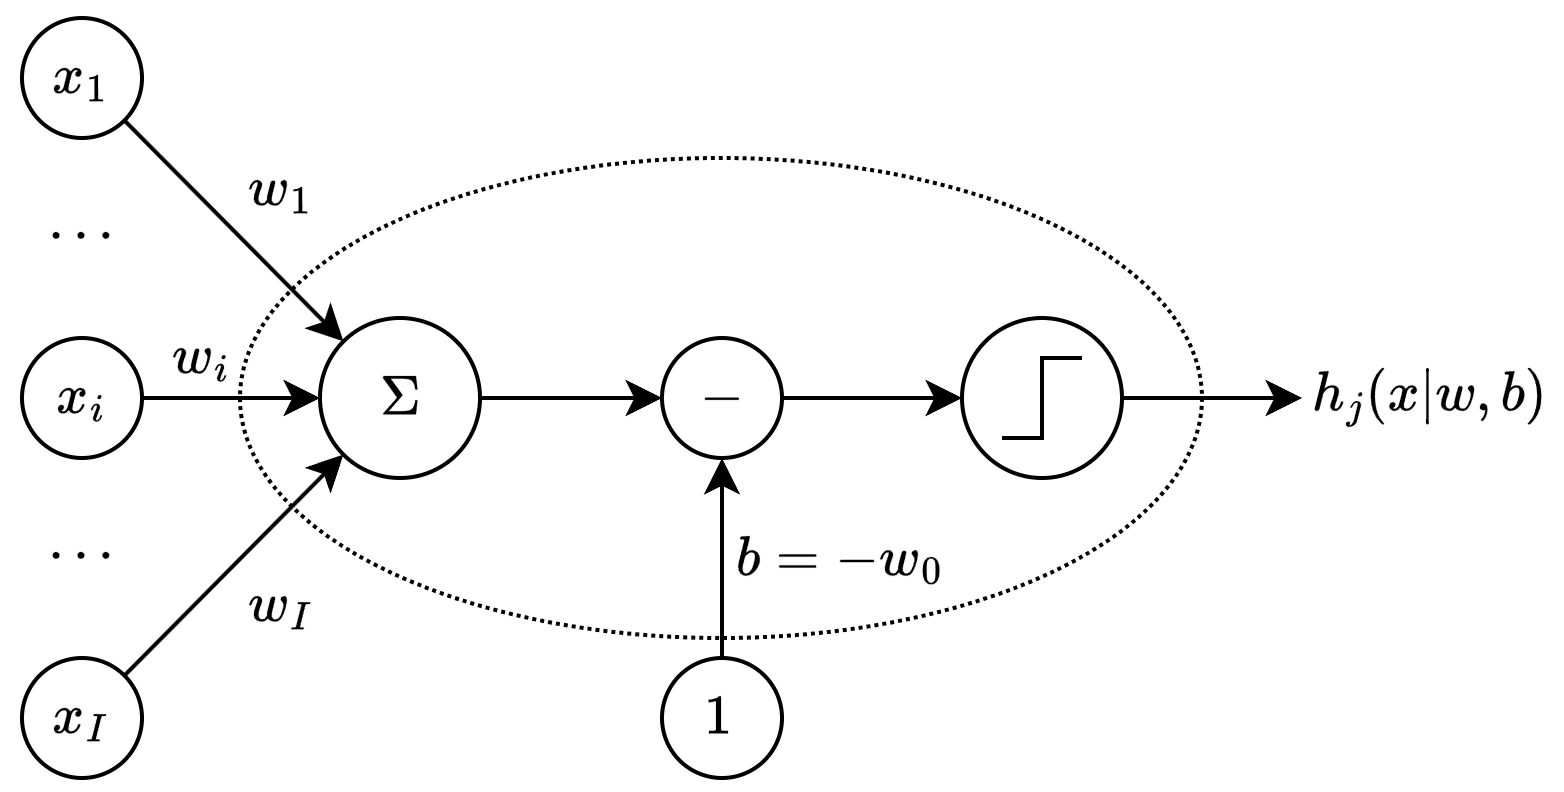
\includegraphics[width=0.75\linewidth]{images/neuron.png}
    \caption{Artificial neuron}
\end{figure}
\noindent The output function $h_j(\mathbf{x}|\mathbf{w},b)$ is given by:
\[h_j(\mathbf{x}|\mathbf{w},b)=h_j\left(\sum_{i=1}^Iw_ix_i-b\right)=h_j\left(\sum_{i=0}^Iw_ix_i\right)=h_j\left(\mathbf{w}^T\mathbf{x}\right)\]
\noindent The activation function in an artificial neuron can take various forms, such as a step function (outputting values between 0 and 1) or a sine function (outputting values between -1 and 1).

The Perceptron computes a weighted sum of its inputs and applies a thresholding function to produce its output:
\[h_j(\mathbf{x}\mid\mathbf{w})=h_j\left(\mathbf{w}^T\mathbf{x}\right)=\text{Sign}(\mathbf{w}^T\mathbf{x})\]
This defines a linear classifier, where the decision boundary is a hyperplane described by:
\[\mathbf{w}^T\mathbf{x}=0\]
The linear decision boundary enables the Perceptron to implement Boolean logic operators. 
However, the Perceptron struggles when data cannot be separated by a linear boundary.
In such cases, additional strategies are necessary. 
These challenges paved the way for more advanced models, such as Multi-Layer Perceptrons.

\paragraph*{Hebbian learning}
Hebbian learning, often summarized by the phrase cells that fire together, wire together, follows these principles:
\begin{enumerate}
    \item Initialize weights randomly.
    \item Adjust weights for each sample (online learning), but only if the sample is misclassified.
\end{enumerate}
The weight update rule is given by:
\[w_i^{k+1}=w_i^k+\eta x_i^kt^k\]
Here, $\eta$ is the learning rate, $x_i^k$ represents the $i$-th input to the Perceptron at time $k$, and $t^k$ is the desired output at the same time. 

    \chapter{Transition systems}
    \section{Introduction}

Sensors serve to detect both the internal condition of the robot (proprioceptive sensors) and the external state of the environment (exteroceptive sensors).

Effectors are responsible for altering the state of the environment, with actuators facilitating the actions of effectors.
    \section{Linear regression}

The goal of regression is to approximate a function $f(x)$ that maps input $x$ to a continuous output $t$ from a dataset $\mathcal{D}$: 
\[\mathcal{D}=\left\{ \left\langle x,t \right\rangle \right\} \implies t=f(x)\]
Here, $x$ is a vector. 
To perform regression, we assume the existence of a function capable of performing this mapping.
The key components of constructing a linear regression problem include:
\begin{itemize}
    \item The method used to model the function $f$ (the hypothesis space). 
    \item The evaluation criteria for the approximation (the loss function).
    \item The optimization process for optimizing the model.
\end{itemize}

In linear regression, the function $f$ is modeled using linear functions. 
This choice is motivated by several factors:
\begin{itemize}
    \item Linear models are easily interpretable, making them suitable for explanation.
    \item Linear regression problems can be solved analytically, allowing for efficient computation.
    \item Linear functions can be extended to model nonlinear relationships.
    \item More sophisticated methods often build upon or incorporate elements of linear regression.
\end{itemize}

\paragraph*{Hypothesis space}
In mathematical terms, the approximation $y$ can be defined as: 
\[y(\textbf{x},\textbf{w})=w_0+\sum_{j=1}^{D-1}w_j x_j=\textbf{w}^T\textbf{x}\]
Here, $\textbf{x} = \left( 1,x_1,\dots,x_{D-1} \right)$ is a vector, and $w_0$ is called the bias parameter.
It's important to note that the output $y$ is a scalar value. 

In a two-dimensional space, our hypothesis space will be the set of all points in the plane $(w_0,w_1)$. 
The coordinates of each point will correspond to a line in the $\left( \textbf{x}, y \right)$ space.

\paragraph*{Loss function}
A commonly used error loss function for the linear regression problem is the sum of squared errors (SSE), defined as:
\[L(\textbf{w})=\dfrac{1}{2}\sum_{n=1}^{N}\left( y(x_n, \textbf{w})-t_n \right)^2\]
This sum is also referred to as the residual sum of squares (RSS) and can be expressed as the sum of squared residual errors:
\[RSS(\textbf{w})=\left\lVert \boldsymbol{\epsilon}^2_2 \right\rVert = \sum_{i=1}^{N}\epsilon^2_i \]
This formulation of the loss function allows for obtaining a closed-form optimization solution.

\paragraph*{Optimization}
For linear models, a closed-form optimization of the RSS, known as least squares, begins with the matrix representation of the loss function:
\[L(\textbf{w})=\dfrac{1}{2}RSS(\textbf{w})=\dfrac{1}{2}\left( \textbf{t}-\boldsymbol{\Phi}_{\textbf{w}} \right)^T\left( \textbf{t}-\boldsymbol{\Phi}_{\textbf{w}} \right)\]
Here, $\boldsymbol{\Phi}=\begin{bmatrix} \phi(x_1) & \dots & \phi(x_N)\end{bmatrix}^T$ and $\textbf{t}=\begin{bmatrix}t_1 & \dots & t_n\end{bmatrix}^T$.
To find the optimal $\textbf{w}$, we compute the first derivative of $L(\textbf{w})$ and set it to zero:
\[\hat{\textbf{w}}_{OLS}=\left( \boldsymbol{\Phi}^T\boldsymbol{\Phi}\right)^{-1}\boldsymbol{\Phi}^T\textbf{t}\]
However, the inversion of the matrix $\boldsymbol{\Phi}^T\boldsymbol{\Phi}^{-1}$ can be computationally expensive, especially for large datasets, with a complexity of $O(nm^2+m^3)$, assuming the matrix is non-singular (invertible). 

To mitigate this, stochastic gradient descent (SGD) can be employed. 
The algorithm known as least mean squares (LMS) uses the following update rule:
\[L(\textbf{x})=\sum_nL(x_n)\]
Expanding this, we get:
\begin{align*}
    \textbf{w}^{(n+1)}  &= \textbf{w}^{(n)}-\alpha^{(n)}\nabla L(x_n) \\
                        &= \textbf{w}^{(n)}-\alpha^{(n)}\left( \textbf{w}^{(n)^T}\phi(\textbf{x}_n)-t_n \right)\phi(\textbf{x}_n)
\end{align*}
Here, $\alpha$ is the learning rate, and convergence is guaranteed if $\sum_{n=0}^{\infty}=+\infty$ and $\sum_{n=0}^{\infty}=\alpha^{(n)^2}<+\infty$.

If the regression problem involves multiple outputs, meaning that $\textbf{t}$ is not a scalar, we can solve each regression problem independently.
However, we can still use the same set of basis functions.
The solution for the weight vectors for all outputs can be expressed as:
\[\hat{\textbf{W}}=\left( \boldsymbol{\Phi}^T\boldsymbol{\Phi}\right)^{-1}\boldsymbol{\Phi}^T\textbf{T}\]
Here, each column of matrix $\textbf{T}$ and $\hat{\textbf{W}}$ corresponds to the target vector and the weight vector for each output, respectively.
This solution can be easily decoupled for each output $k$: 
\[\hat{\textbf{w}}_k=\left( \boldsymbol{\Phi}^T\boldsymbol{\Phi}\right)^{-1}\boldsymbol{\Phi}^T\textbf{t}_k\]
An advantage of this approach is that $\left( \boldsymbol{\Phi}^T\boldsymbol{\Phi}\right)^{-1}$ only needs to be computed once, regardless of the number of outputs.

\subsection{Basis function}
While a linear combination of input variables may not always suffice to model data, we can still construct a regression model that is linear in its parameters. 
This can be achieved by defining a model using non-linear basis functions, expressed as:
\[y(\textbf{x},\textbf{w})=w_0+\sum_{j=1}^{M-1}w_j \phi_j(\textbf{x})=\textbf{w}^T\boldsymbol{\phi}(\textbf{x})\]
Here, the components of the vector  $\boldsymbol{\phi}(\textbf{x})=\left( 1,\phi_1(\textbf{x}),\dots,\phi_{M-1}(\textbf{x}) \right)^T$  are referred to as features.
These features allow for a more flexible representation of the input data, enabling the model to capture non-linear relationships between the input variables and the output.
\begin{example}
    Let's reconsider a set of data regarding individuals' weight and height, along with their completion times for a one-kilometer run:
    \begin{table}[H]
        \centering
        \begin{tabular}{c|c|c}
        \textbf{Height (cm)} & \textbf{Weight (kg)} & \textbf{Completion time (s)} \\ \hline
        180                  & 70                   & 180                          \\
        184                  & 80                   & 220                          \\
        174                  & 60                   & 170                         
        \end{tabular}
    \end{table}
    We can model this problem using a dummy variable and introduce the Body Mass Index (BMI) as a new feature:
    \begin{table}[H]
        \centering
        \begin{tabular}{c|c|c|c|c}
        \textbf{Dummy variable} & \textbf{Height (cm)} & \textbf{Weight (kg)} & \textbf{BMI} & \textbf{Completion time (s)} \\ \hline
        $x_0$                   & $x_1$                & $x_2$                & $x_3$        & $t$                          \\
        1                       & 180                  & 70                   & 21           & 180                          \\
        1                       & 184                  & 80                   & 23           & 220                          \\
        1                       & 174                  & 60                   & 20           & 170                         
        \end{tabular}
    \end{table}
    Here, the dummy variable $x_0$ is always initialized to one.
    Now, we have the option to retain or discard the weight and height variables, considering only the BMI values for analysis.
\end{example}
The most commonly used basis functions in regression are:
\begin{itemize}
    \item \textit{Polynomial}: 
        \[\phi_j(x)=x^j\]
    \item \textit{Gaussian}:
        \[\phi_j(x)=\exp \left( -\dfrac{\left( x-\mu_j \right)^2}{2 \sigma^2} \right) \]
    \item \textit{Sigmoidal}: 
        \[\phi_j(x)=\dfrac{1}{1+\exp\left(\dfrac{\mu_j-x}{\sigma}\right)}\]
\end{itemize}
Here, the constant $\mu_j$ is referred to as a hyperparameter, as its value needs to be determined through experimentation and depends on the user's experience.

\begin{figure}[H]
    \centering
    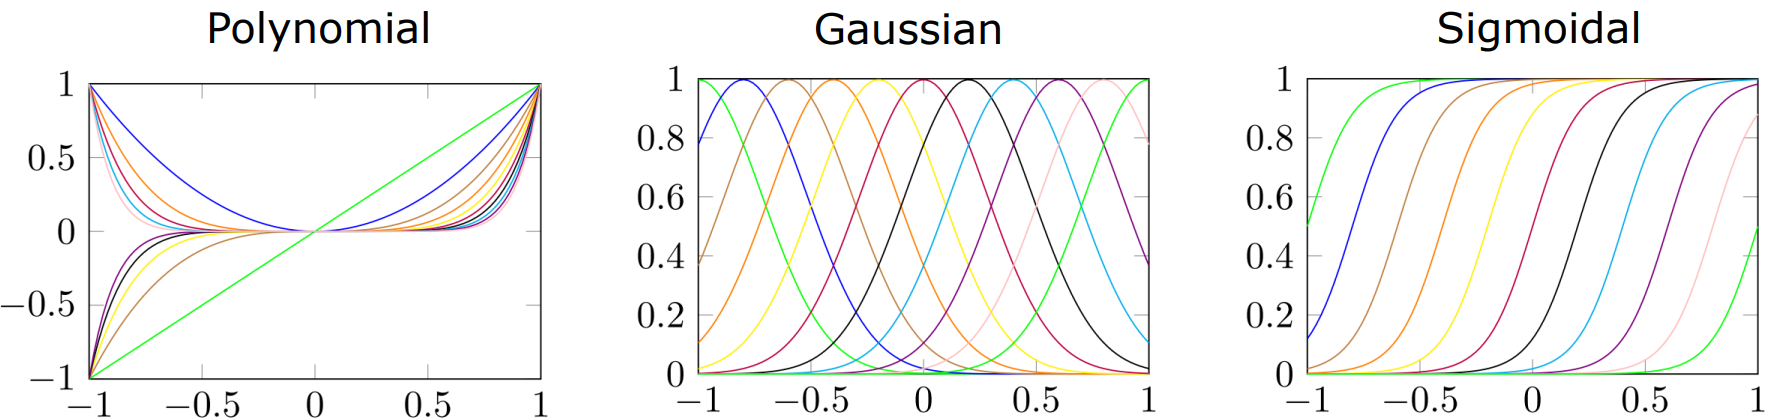
\includegraphics[width=0.75\linewidth]{images/basis.png}
    \caption{Some possible basis functions shapes}
\end{figure}

It's noteworthy that the Gaussian basis function allows for a local approximation by omitting values that are close to zero.
This approach enables capturing the relationship between the input and output in a reduced input space area.
As we move away from the mean, approaching zero, the values become negligible.

\subsection{Regularization}
A function can achieve a better approximation by increasing the degree of the polynomial used in the regression.
\begin{example}
    Consider a function generating a set of points with some noise:
    \begin{figure}[H]
        \centering
        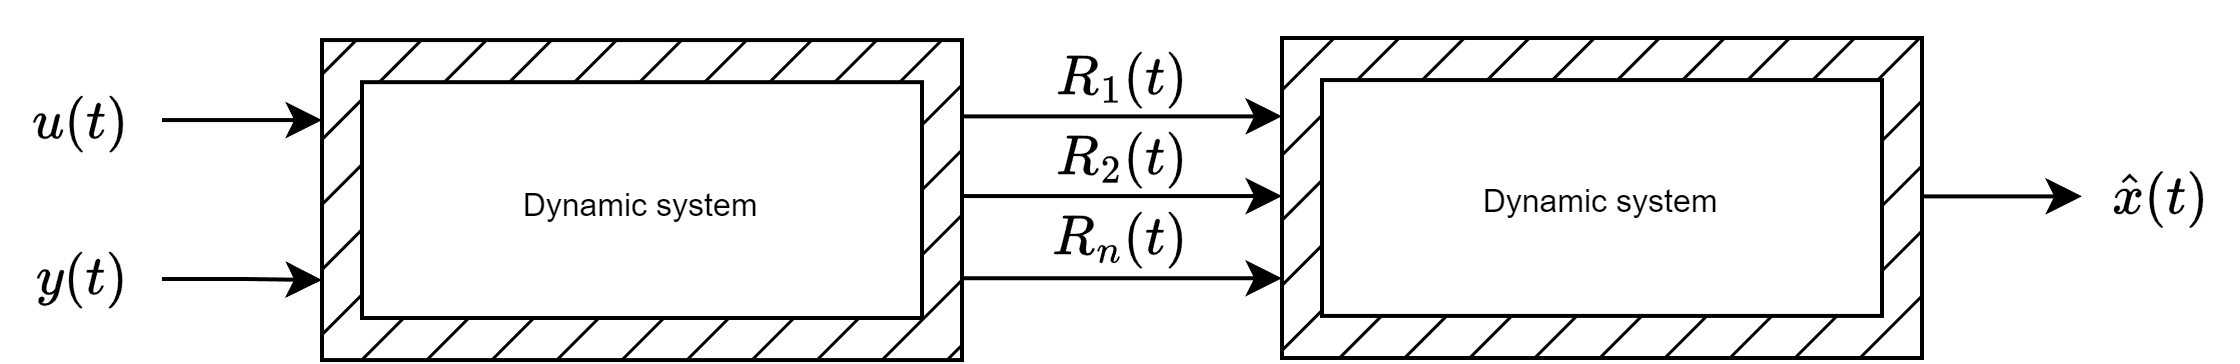
\includegraphics[width=0.25\linewidth]{images/reg.png}
    \end{figure}
    Using a second-order polynomial instead of a linear one provides a better approximation:
    \begin{figure}[H]
        \centering
        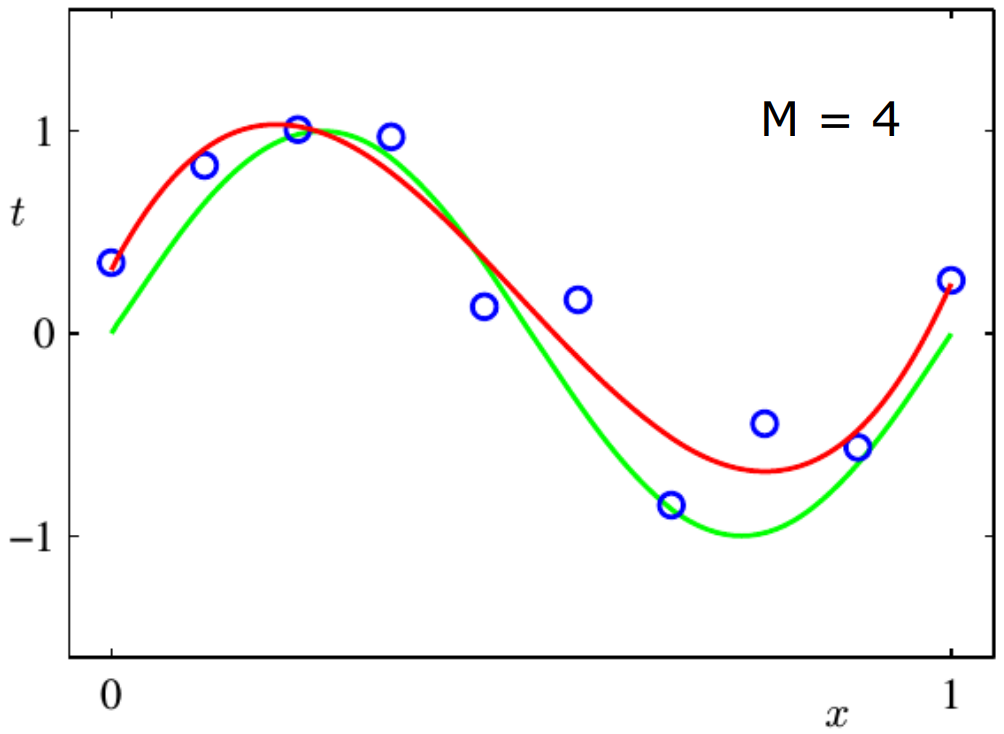
\includegraphics[width=0.25\linewidth]{images/reg1.png}
    \end{figure}
    Further improving the approximation can be achieved with a higher-degree polynomial (e.g., ninth grade):
    \begin{figure}[H]
        \centering
        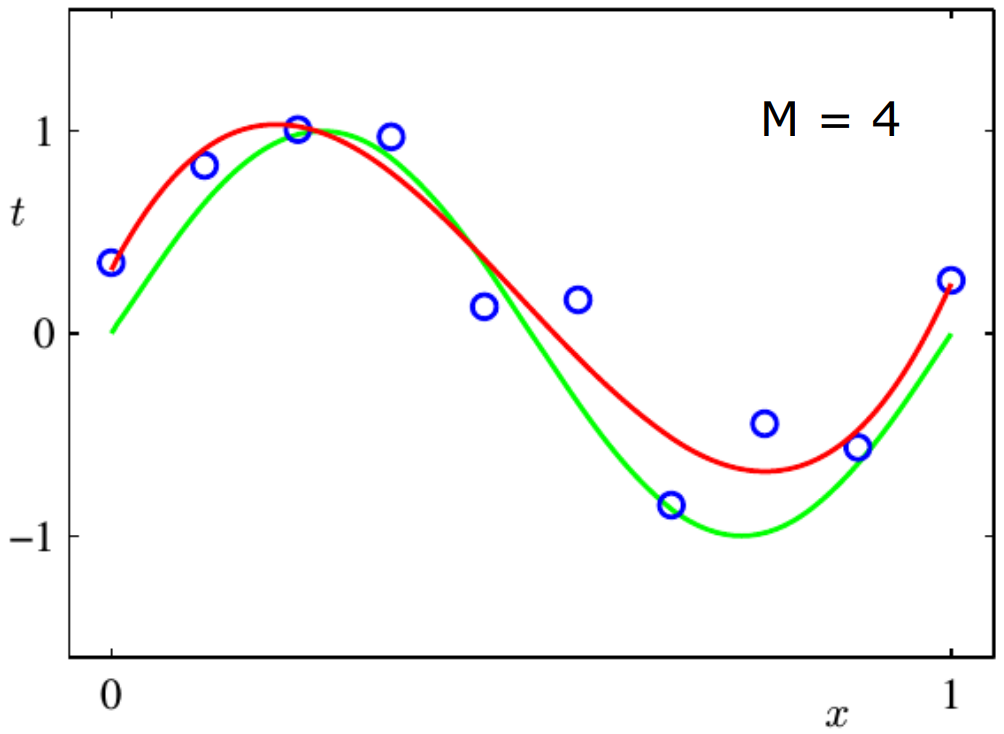
\includegraphics[width=0.25\linewidth]{images/reg1.png}
    \end{figure}
\end{example}
However, increasing the polynomial degree also increases the complexity of the model parameters.
To address this complexity, adjustments are needed in the loss function:
\[L(\textbf{w})=L_D(\textbf{w})+\lambda L_W(\textbf{w})\]
Here, $L_D(\textbf{w})$ represents the usual loss function, $L_W(\textbf{w})$ reflects model complexity (a hyperparameter), and $\lambda$ is the regularization coefficient.
$L_W(\textbf{w})$ can be tailored using ridge regression or lasso methods.

\paragraph*{Ridge regression}
In ridge regression, the regularization term $L_W(\textbf{w})$ is defined as:
\[L_W(\textbf{w})=\dfrac{1}{2}\textbf{w}^T\textbf{w}=\dfrac{1}{2}\left\lVert \textbf{w} \right\rVert_2^2 \]
Thus, the overall loss function becomes:
\[L(\textbf{w})=\dfrac{1}{2}\sum_{i=1}^N \left( t_i-\textbf{w}^T\phi(x_i) \right)^2 + \dfrac{\lambda}{2}\left\lVert \textbf{w} \right\rVert_2^2\]
Despite the regularization term, the loss function remains quadratic with respect to $w$, allowing for closed-form optimization:
\[\hat{\textbf{w}}_{ridge}=\left( \lambda\textbf{I}+\boldsymbol{\Phi}^T \boldsymbol{\Phi} \right)^{-1}\boldsymbol{\Phi}^T\text{t}\]
The term $\lambda\textbf{I}$ is crucial in solving the singularity problem, as it transforms a non-singular matrix into a singular one with an appropriate choice of $\lambda$. 

\paragraph*{Lasso}
Another common regularization method is lasso, where the regularization term $L_W(\textbf{w})$ is defined as:
\[L_W(\textbf{w})=\dfrac{1}{2}\left\lVert \textbf{w} \right\rVert_1=\dfrac{1}{2}\sum_{j=0}^{M-1}\left\lvert w_j \right\rvert\]
Thus, the overall loss function becomes:
\[L(\textbf{w})=\dfrac{1}{2}\sum_{i=1}^N \left( t_i-\textbf{w}^T\phi(x_i) \right)^2 + \dfrac{\lambda}{2}\left\lVert \textbf{w} \right\rVert_1\]
In this case, closed-form optimization is not possible. 
However, lasso typically leads to sparse regression models: when the regularization coefficient $\lambda$ is large enough, some components of $\hat{\textbf{w}}$ become equal to zero.
Regularization can be seen as equivalent to minimizing  $L_D(\textbf{w})$ subject to the constraint:
\[\sum_{j=0}^{M-1}\left\lvert w_j \right\rvert \leq \eta\] 

\subsection{Linear regression with probability}
We can approach regression in a probabilistic manner by defining a model that probabilistically maps inputs ($x$) to outputs ($t$).
This model, denoted as $y(x, w)$, incorporates unknown parameters ($w$).
We then model the likelihood, i.e., the probability that observed data $\mathcal{D}$ is generated by a given set of parameters ($w$), as: 
\[\text{P}(\mathcal{D}|\textbf{w})\]
Finally, we estimate the parameters ($w$) by maximizing the likelihood:
\[\textbf{w}_{ML}=\argmax_{\textbf{w}}\text{P}(\mathcal{D}|\textbf{w})\]

For linear regression, we define the model as:
\[t=y(\textbf{x},\textbf{w})+\epsilon=\textbf{w}^T\boldsymbol{\Phi}(\textbf{x})+\epsilon\]
Here, we assume a linear model for $y(\textbf{x},\textbf{w})$ and introduce noise  $\epsilon\sim\mathcal{N}(0,\sigma^2)$. 
Consequently, given a dataset $\mathcal{D}$ of $N$ samples with inputs $\textbf{X}=\begin{bmatrix}\textbf{x}_1 & \dots & \textbf{x}_n \end{bmatrix}$ and outputs $\textbf{t}=\begin{bmatrix}t_1 & \dots & t_n \end{bmatrix}^T$, we have: 
\[\text{P}(\mathcal{D}|\textbf{w})=\text{P}(\textbf{t}|\textbf{X},\textbf{w},\sigma^2)=\prod_{n=1}^{N}\mathcal{N}(t_n|\textbf{w}^T\boldsymbol{\Phi}(\textbf{x}_n),\sigma^2)\]
 
To find $\textbf{w}_{ML}$, it is convenient to maximize the log-likelihood, obtaining:
\[\ell (\textbf{w})=\ln\text{P}(t_n|\textbf{x}_n, \textbf{w} ,\sigma^2)=-\dfrac{N}{2}\ln(2\pi\sigma^2)-\dfrac{1}{2\sigma^2}RSS(\textbf{w})\]
Notice that the first part of the final formula is a constant independent of $\textbf{w}$, so it can be ignored in maximizing the likelihood.
Solving the optimization problem by setting the gradient to zero $\ell (\textbf{w})=0$, yields the final formula:
\[\textbf{w}_{ML}=\left( \boldsymbol{\Phi}^T\boldsymbol{\Phi} \right)^{-1}\boldsymbol{\Phi}^T\textbf{t}\]
This result aligns with the ordinary least squares approach.

This outcome allows us to interpret ordinary least squares from a probabilistic perspective, confirming that we are utilizing a normally distributed probabilistic function to generate the residuals in OLS.

\paragraph*{Bayesian linear regression}
Bayesian linear regression follows a structured approach:
\begin{enumerate}
    \item Formulation of probabilistic knowledge:
        \begin{enumerate}
            \item Qualitatively define the model expressing our knowledge.
            \item Incorporate unknown parameters into the model.
            \item Represent assumptions about these parameters with a prior distribution before observing any data.
        \end{enumerate}
    \item Data observation.
    \item Computation of posterior probability distribution for parameters:
        \[\text{P}(parameters|data)=\dfrac{\text{P}(data|parameters)\text{P}(parameters)}{\text{P}(data)}\]
    \item Utilization of Posterior Distribution to:
        \begin{itemize}
            \item Make predictions by averaging over the posterior distribution.
            \item Assess or accommodate uncertainty in parameter values.
            \item Make decisions by minimizing expected posterior loss.
        \end{itemize}
\end{enumerate}

The posterior distribution for model parameters is derived by combining the prior with the likelihood for parameters given the data:
\[\text{P}(\textbf{w}|\mathcal{D})=\dfrac{\text{P}(\mathcal{D}|\textbf{w})\text{P}(\textbf{w})}{\text{P}(\mathcal{D})}\]
Here, $\text{P}(\textbf{w})$ represents the prior probability over parameters, $\text{P}(\mathcal{D}|\textbf{w})$ denotes the likelihood, and $\text{P}(\mathcal{D})$ is the marginal likelihood acting as a normalization constant: 
\[\text{P}(\mathcal{D})=\int\text{P}(\mathcal{D}|\textbf{w})\text{P}(\textbf{w})d\textbf{w}\] 

The mode of the posterior, known as the Maximum A Posteriori (MAP) estimate, yields the most probable value of $\textbf{w}$ given the data.

A Gaussian likelihood assumption allows the prior to be modeled conveniently as a conjugate prior:
\[\text{P}(\textbf{w})=\mathcal{N}(\textbf{w}|\textbf{w}_0,\textbf{S}_0)\]
Consequently, the posterior remains Gaussian:
\[\text{P}(\textbf{w}|\textbf{t},\boldsymbol{\Phi},\sigma^2)\varpropto \mathcal{N}(\textbf{w}|\textbf{w}_0,\textbf{S}_0)\mathcal{N}(\textbf{t}|\boldsymbol{\Phi}\textbf{w},\sigma^2\textbf{I})\]
Resulting in:
\[\begin{cases}
    \text{P}(\textbf{w}|\textbf{t},\boldsymbol{\Phi},\sigma^2)=\mathcal{N}(\textbf{w}|\textbf{w}_N,\textbf{S}_N) \\
    \textbf{w}_N=\textbf{S}_N\left(\textbf{S}_0^{-1}\textbf{w}_0+\dfrac{\boldsymbol{\Phi}^T\textbf{t}}{\sigma^2}\right) \\
    \textbf{S}_N^{-1}=\textbf{S}_0^{-1}+\dfrac{\boldsymbol{\Phi}^T\boldsymbol{\Phi}}{\sigma^2}
\end{cases}\]

\paragraph*{Prior infinitely broad}
When the prior distribution is infinitely broad, the Maximum A Posteriori (MAP) estimate coincides with the Maximum Likelihood (ML) solution:
\[\begin{cases}
    \lim_{\textbf{S}_0\rightarrow\infty}\textbf{w}_N=\left( \boldsymbol{\Phi}^T\boldsymbol{\Phi} \right)^{-1}\boldsymbol{\Phi}^T\textbf{t} \\
    \lim_{\textbf{S}_0\rightarrow\infty}\textbf{S}_N^{-1}=\dfrac{\boldsymbol{\Phi}^T\boldsymbol{\Phi}}{\sigma^2}
\end{cases}\]
This yields the ordinary least squares formula.
However, in this case, we also have the covariance matrix, providing information about the related uncertainty.
The only missing parameter is $\sigma^2$, which can be computed as:
\[\sigma^2=\dfrac{1}{N-M}\sum_{n=1}^{N}\left( t_n-\hat{\textbf{w}}^T\boldsymbol(\phi)(\textbf{x}_n) \right)^2\]
The ML estimate $\textbf{w}_{ML}$ of $\textbf{w}$ has the smallest variance among linear unbiased estimates and the lowest Mean Squared Error (MSE) among linear unbiased estimates (Gauss-Markov).

\paragraph*{Prior not infinitely broad}
When the prior distribution is not infinitely broad, such that $\textbf{w}_0=0$ and $\textbf{S}_0=\tau^2\textbf{I}$, we can express the logarithm of the posterior distribution $\text{P}(\textbf{w}|\textbf{t})$ as:
\[\ln\text{P}(\textbf{w}|\textbf{t})=-\dfrac{1}{2\sigma^2}\sum_{i=1}^{N}\left(t_i-\textbf{w}^T\boldsymbol{\phi}(\textbf{x}_i)\right)^2-\dfrac{1}{2\tau^2}\left\lVert \textbf{w}\right\rVert_2^2 \]
In this scenario, the Maximum A Posteriori estimate, MAP($\textbf{w}N$), coincides with the solution of ridge regression $\hat{\textbf{w}}{ridge}$ with a regularization parameter $\lambda$ set to $\lambda=\frac{\sigma^2}{\tau^2}$.

\paragraph*{Sequential learning}
How to leverage the Bayesian approach for sequential learning:
\begin{enumerate}
    \item Begin by computing the posterior with the initial data.
    \item As additional data becomes available, update the prior with this new information to obtain the updated posterior.
\end{enumerate}

\paragraph*{Predictive distribution}
In a Bayesian framework, one can determine the probability distribution of the target variable for a new sample $\textbf{x}^\ast$ (given the training data $\mathcal{D}$) by integrating over the posterior distribution:
\[\text{P}(t^\ast|\textbf{x}^\ast,\mathcal{D})=\mathbb{E}\left[ t^\ast|\textbf{x}^\ast,\textbf{w},\mathcal{D} \right] = \int\text{P}(t^\ast|\textbf{x}^\ast,\textbf{w},\mathcal{D})\text{P}(\textbf{w}|\mathcal{D})d\textbf{w}\]
This is commonly referred to as the predictive distribution.
However, computing this predictive distribution typically involves the intractable task of determining the posterior distribution.
Nevertheless, under certain assumptions, it is possible to compute the predictive distribution as follows: 
\[\sigma_N^2(\textbf{x})=\sigma^2+\boldsymbol{\phi}(\textbf{x})^T\textbf{S}_N\boldsymbol{\phi}(\textbf{x})\]
Here, as the number of data points $N$ approaches infinity, the uncertainty associated with the parameters (second term) diminishes, and the variance of the predictive distribution depends solely on the variance of the data ($\sigma^2$). 

\subsection{Challenges and limitations}
Modeling presents challenges in ensuring our model effectively represents a wide range of plausible functions while maintaining informative priors without overly spreading out probabilities or assigning negligible values.

On the computational side, limitations arise with analytical integration, particularly in cases involving non-conjugate priors and complex models. 
Approaches like Gaussian (Laplace) approximation, Monte Carlo integration, and variational approximation become necessary for addressing these complexities and achieving accurate results.

Linear models with fixed basis functions offer several benefits:
\begin{itemize}
    \item They permit closed-form solutions, facilitating efficient computation.
    \item They lend themselves to tractable Bayesian treatment, enabling principled uncertainty quantification.
    \item They can capture non-linear relationships by employing appropriate basis functions.
\end{itemize}
However, these models also come with several drawbacks:
\begin{itemize}
    \item Basis functions remain static and non-adaptive to variations in the training data.
    \item These models are susceptible to the curse of dimensionality, particularly when dealing with high-dimensional feature spaces.
\end{itemize}
    \section{Classification}














    \section{Multiple scanners}

Sometimes is useful to have more than one scanner together. 
To facilitate the support for multiple scanners, the following methods are employed:
\begin{itemize}
    \item Rules can be designated with the name of the associated scanner, known as the start condition.
    \item Special actions enable the transition between scanners.
\end{itemize}

A start condition, denoted by \texttt{S} is utilized to annotate rules as \texttt{<S>RULE} and activate rules when the scanner operates in the \texttt{S} start condition.
Start conditions can be:
\begin{itemize}
    \item \textit{Exclusive}, declared with \texttt{$\%$x S}; this disables unmarked rules when the scanner operates in the \texttt{S} start condition.
    \item \textit{Inclusive}, declared with \texttt{$\%$s S}; unmarked rules are active when the scanner operates in the \texttt{S} start condition.
\end{itemize}
The initial condition is inclusive by default.
Additionally:
\begin{itemize}
    \item The \texttt{*} start condition matches any start condition.
    \item The initial start condition is denoted as \texttt{INITIAL}.
    \item Start conditions are represented as integers.
    \item The current start condition is stored in the \texttt{YY$\_$START} variable.
\end{itemize}
    \section{Skyline queries}

Skyline queries aim to identify superior objects across multiple perspectives, relying on the concept of dominance.
\begin{definition}[\textit{Domination}]
    A tuple $t$ dominates a tuple $s$ ($t \prec s$) if and only if $t$ in nowhere worse than $s$: 
    \[\forall i, 1 \leq i \leq m \rightarrow t[A_i] \leq s[A_i]\] 
    And is better at least once: 
    \[\exists j, 1 \leq j \leq m \land t[A_j] < s[A_j]\]
\end{definition}
\begin{definition}[\textit{Skyline}]    
    The skyline of a relation is the set of its non-dominated tuples.
\end{definition}

The convention on the skyline queries is that lower values are better than higher values.
The convention is that lower values are considered better. 
A tuple is part of the skyline if it is the top-1 result with respect to at least one monotone scoring function. 

\paragraph*{Query syntax}
The syntax for skyline queries can be expressed as follows:
\begin{lstlisting}[style=SQL]
SELECT <attributes>
FROM R1,R2,...,Rn
WHERE <conditions>
GROUP BY <conditions>
HAVING <conditions>
SKYLINE OF [DISTINCT] d1[MIN|MAX|DIFF], ..., dm[MIN|MAX|DIFF]
ORDER BY <conditions>
\end{lstlisting}
This query can be easily translated into a standard query, but the result is too slow and cannot be used in practice. 

\subsection{Block Nested Loop algorithm}
The Block Nested Loop algorithm takes a dataset $D$ of multidimensional points as input and outputs the skyline of $D$. 
Its complexity is $O(n^2)$, making it inefficient for large datasets.
\begin{algorithm}[H]
    \caption{Block nested loop algorithm}
        \begin{algorithmic}[1]
            \State $W \leftarrow \varnothing$
            \For {every point $p$ in $D$}
                \If {$p$ not dominated by any point in $W$}
                    \State remove from $W$ the points dominated by $p$
                    \State add $p$ to $W$
                \EndIf
            \EndFor
            \State \Return $W$
        \end{algorithmic}
\end{algorithm}

\subsection{Sort Filter Skyline algorithm}
The Sort Filter Skyline algorithm also takes a dataset $D$ of multidimensional points as input and outputs the skyline of $D$. 
It performs better than the Block Nested Loop algorithm, especially for large datasets, but still has a complexity of $O(n^2)$.
\begin{algorithm}[H]
    \caption{Sort filter skyline algorithm}
        \begin{algorithmic}[1]
            \State $S \leftarrow D$
            \State $W \leftarrow \varnothing$
            \For {every point $p$ in $S$}
                \If {$p$ not dominated by any point in $W$}
                    \State add $p$ to $W$
                \EndIf
            \EndFor
            \State \Return $W$
        \end{algorithmic}
\end{algorithm}
\begin{example}
    Consider the following unordered dataset: 
    \begin{table}[H]
        \centering
        \begin{tabular}{lcc}
        \textbf{Name}                 & \textbf{Cost} & \textbf{Complaints} \\ \hline
        \multicolumn{1}{l|}{Crillon}  & 0.25  & 0.1        \\
        \multicolumn{1}{l|}{Ibis}     & 0.08  & 0.3        \\
        \multicolumn{1}{l|}{Hilton}   & 0.175 & 0.3        \\
        \multicolumn{1}{l|}{Sheraton} & 0.2   & 0.2        \\
        \multicolumn{1}{l|}{Novotel}  & 0.15  & 0.1       
        \end{tabular}
    \end{table}
    The skyline, consisting of Novotel and Ibis, is identified by the algorithm.
\end{example}

\subsection{Summary}
Skyline queries are effective in identifying potentially interesting objects when user preferences are unknown. 
They are simple to use but return a large number of objects, and their computation is not highly efficient. 
Skyline queries are agnostic with respect to user preferences.

\paragraph*{K-skyband} 
To enhance skyline queries, the concept of $k$-skyband is introduced, where the result includes a set of tuples dominated by fewer than $k$ tuples.
    \section{ARMA process}

We can define a process that combines elements from both the AutoRegressive and Moving Average processes as follows:
\[y(t)=a_1y(t-1)+a_2y(t-2)+\cdots+a_m y(t-m)+c_0e(t)+c_1e(t-1)+\cdots+c_n e(t-n) \]
Here, $e(t)\sim WN(0,\lambda^2)$.

This process comprises two components: one being the AR($m$) process and the other being the MA($n$) process. 
It is denoted as an ARMA($m,n$) process.
Since it combines elements from two distinct processes, we can make the following observations:
\begin{itemize}
    \item The MA($n$) process is equivalent to an ARMA($0,n$) process.
    \item The AR($m$) process is equivalent to an ARMA($m,0$) process. 
\end{itemize}
\begin{figure}[H]
    \centering
    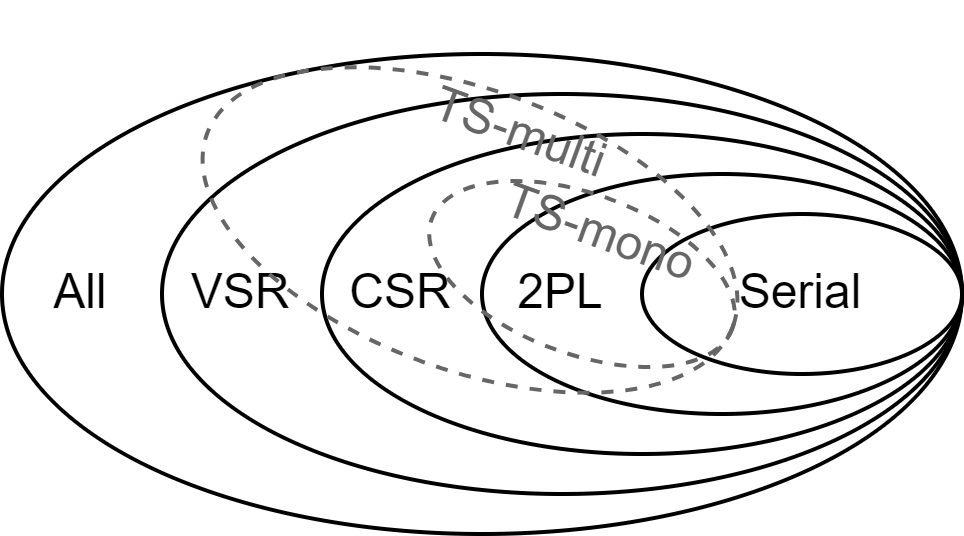
\includegraphics[width=0.45\linewidth]{images/set.png}
    \caption{Inclusion of ARMA processes}
\end{figure}

\subsection{Operatorial representation}
Given an ARMA($m,n$) process defined as:
\[y(t)=a_1y(t-1)+a_2y(t-2)+\cdots+a_m y(t-m)+c_0e(t)+c_1e(t-1)+\cdots+c_n e(t-n)\]
Here, $e(t)\sim WN(0,\lambda^2)$.

We can rewrite it using operatorial representation as:
\[y(t)=a_1z^{-1}y(t)+a_2z^{-2}y(t)+\cdots+a_m z^{-m}y(t)+c_0e(t)+c_1z^{-1}e(t)+\cdots+c_n z^{-n}e(t)\]
Rearranging terms, we get:
\[\left(1- a_1z^{-1}-a_2z^{-2}-\cdots-a_m z^{-m}\right)y(t)=\left(c_0+c_1z^{-1}+\cdots+c_n z^{-n}\right)e(t)\]
Finally, we can express $y(t)$ in terms of $e(t)$ using the transfer function notation:
\[y(t)=\dfrac{c_0+c_1z^{-1}+\cdots+c_n z^{-n}}{1- a_1z^{-1}-a_2z^{-2}-\cdots-a_m z^{-m}}e(t)=\dfrac{C(z)}{A(z)}e(t)\]
Here, $C(z)$ and $A(z)$ are polynomials representing the coefficients of the Moving Average and AR parts, respectively. 
This ratio, denoted as $W(z)$, is a discrete-time transfer function. 
This operator acts as a digital filter, transforming the input noise sequence $e(t)$ into the output sequence $y(t)$.

\subsection{Mean value}
Given an ARMA($m,n$) model defined as:
\[y(t)=a_1y(t-1)+a_2y(t-2)+\cdots+a_m y(t-m)+c_0e(t)+c_1e(t-1)+\cdots+c_n e(t-n)\]
where $e(t)\sim WN(0,\lambda^2)$, we can compute its mean as follows:
\begin{align*}
    \mathbb{E}\left[y(t)\right] &= \mathbb{E}\left[a_1y(t-1)+\cdots+a_m y(t-m)+c_0e(t)+\cdots+c_n e(t-n)\right] \\
                                &= a_1\mathbb{E}\left[y(t-1)\right]+\cdots+a_m\mathbb{E}\left[y(t-m)\right] +c_0\underbrace{\mathbb{E}\left[e(t)\right]}_0 +\cdots+c_n\underbrace{\mathbb{E}\left[e(t-n)\right]}_0
\end{align*}
Under the assumption that $a_1,a_2,\dots,a_m$ are chosen such that $y(t)$ constitutes a stationary stochastic process, thus exhibiting a constant mean value, we can simplify the above to:
\[m_y=a_1m_y+a_2m_y+\cdots+a_m m_y \rightarrow m_y=0\]

\subsection{Covariance function}
Given an ARMA($m,n$) model defined as:
\[y(t)=a_1y(t-1)+a_2y(t-2)+\cdots+a_m y(t-m)+c_0e(t)+c_1e(t-1)+\cdots+c_n e(t-n)\]
where $e(t)\sim WN(0,\lambda^2)$, we aim to compute the covariance function at $\tau=0$, considering $m_y=0$:
\begin{align*}
    \gamma_y(0) &=\mathbb{E}\left[ \left(y(t)-m_y\right)\left(y(t)-m_y\right) \right] \\
                &=\mathbb{E}\left[ {\left(y(t)\right)}^2 \right] \\
                &=\mathbb{E}\left[ {\left(a_1y(t-1)+\cdots+a_m y(t-m)+c_0e(t)+\cdots+c_n e(t-n)\right)}^2 \right] \\      
                &=a_1^2\underbrace{\mathbb{E}\left[ {y(t-1)}^2 \right]}_{\gamma_y(0)} +\cdots+c_0^2\underbrace{\mathbb{E}\left[ {e(t)}^2 \right]}_{\lambda^2} +\cdots+c_n^2 \underbrace{\mathbb{E}\left[ {e(t-n)}^2 \right]}_{\lambda^2}  +\\
                &+ 2a_1a_2\underbrace{\mathbb{E}\left[ y(t-1)y(t-2) \right]}_{\gamma_y(1)}  + \cdots + 2a_1c_0\underbrace{\mathbb{E}\left[ y(t-1)e(t) \right]}_{0 \text{ if the times are different}}  + \cdots + 2c_0c_1\underbrace{\mathbb{E}\left[ e(t)e(t-1) \right]}_0  \\   
                &=a_1^2\gamma_y(0) +\cdots+c_0^2\lambda^2 +\cdots+c_n^2 \lambda^2  + 2a_1a_2\gamma_y(1)  + \cdots + 2a_1c_1\mathbb{E}\left[ y(t-1)e(t-1) \right]+\dots    
\end{align*}
We require $\gamma_y(1),\gamma_y(2),\dots,\gamma_y(n)$ to compute $\gamma_y(0)$.

To compute the covariance function at $\tau=1$, considering $m_y=0$, we have:
\begin{align*}
    \gamma_y(1) &=\mathbb{E}\left[ \left(y(t)-m_y\right)\left(y(t-1)-m_y\right) \right] \\
                &=\mathbb{E}\left[ \left(a_1y(t-1)+\cdots+a_m y(t-m)+c_0e(t)+\cdots+c_n e(t-n)\right)y(t-1) \right] \\
                &=a_1\mathbb{E}\left[{y(t-1)}^2\right]+\cdots+c_0\mathbb{E}\left[e(t)y(t-1)\right]+\dots \\
                &=a_1\gamma_y(0)+\cdots+c_0\mathbb{E}\left[e(t)y(t-1)\right]+\dots
\end{align*}
Proceeding with increasing values of $\tau$, we obtain a set of $m$ recursive equations known as Yule-Walker equations for an ARMA($m,n$) process:
\[\begin{cases}
    \gamma_y(0)=a_1^2\gamma_y(0) +a_2^2\gamma_y(0) +2a_1a_2\gamma_y(1) +\dots \\
    \gamma_y(1)=a_1\gamma_y(0) +c_0\mathbb{E}\left[e(t)y(t-1)\right] +\dots \\
    \vdots \\
    \gamma_y(m-1)=a_1\gamma_y(m-2)+\dots
\end{cases}\]
At the end we get a set of $m$ recursive equations called Yule-Walker equations for an ARMA($m,n$) process.
These equations require all covariances $\gamma_y(0),\gamma_y(1),\dots,\gamma_y(m-1)$ to compute $\gamma_y(m)$.

    \chapter{Model checking}
    \section{Manufacturing company}

\begin{definition}[\textit{Information intensity}]
    Information intensity refers to the amount and complexity of information required in an organization's processes. 
\end{definition}
\noindent Generally, service industries require higher information intensity than manufacturing.
IT Intensity measures how well IT systems meet an organization's information processing needs. 
However, IT intensity can sometimes be greater in manufacturing than in services, depending on automation and digital integration.
\begin{definition}[\textit{Management inclination}]
    Management inclination reflects how much a company's leadership views IT as a strategic asset. 
\end{definition}
\noindent This varies based on factors like digital literacy, organizational culture, and company history.
Historically, manufacturing companies have adopted IT earlier, while service industries experienced a lag of around ten years.

\paragraph*{Drivers}
Several factors determine how IT intensive a company or industry can be:
\begin{enumerate}
    \item \textit{Structure of information processes}: the more structured and rule-based an activity is, the easier it is to automate using IT.
    \item \textit{Data volume}: the sheer amount of information that needs to be processed influences IT requirements.
    \item \textit{Operational frequency}: tasks that are repeated frequently benefit more from IT automation.
    \item \textit{Computational complexity}: simpler processes are easier to digitize and automate efficiently.
\end{enumerate}

\subsection{Manufacturing value chain}
Porter's value chain concept highlights how IT supports various business activities to create competitive advantages.
\begin{figure}[H]
    \centering
    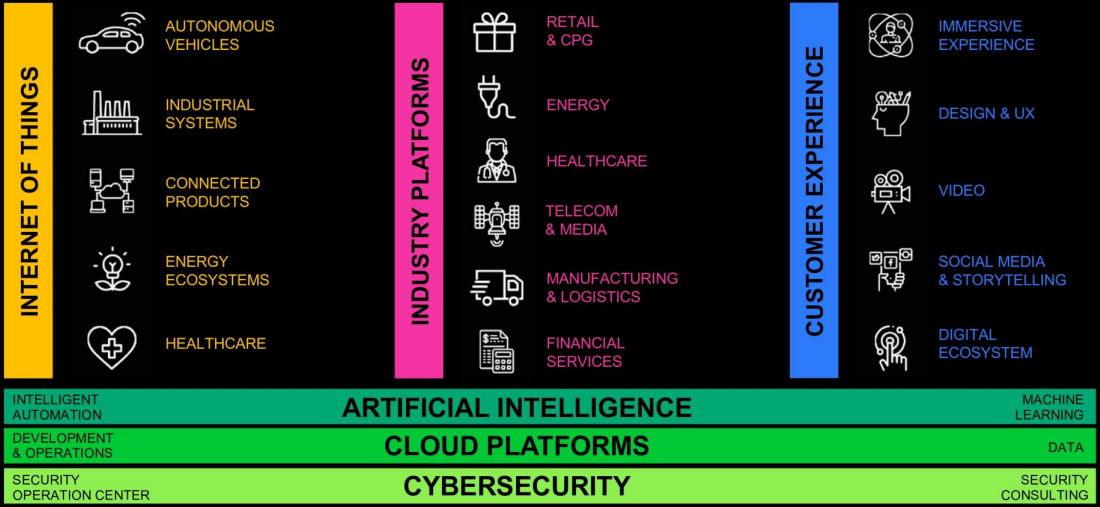
\includegraphics[width=0.75\linewidth]{images/bis2.png}
    \caption{Porter value chain}
\end{figure}

\paragraph*{Activity cycles}
Manufacturing involves continuous, iterative cycles that ensure efficiency and product quality. 
These cycles include:
\begin{enumerate}
    \item \textit{Development cycle}: focuses on designing and industrializing both products and production processes.
    \item \textit{Logistics cycle}: manages customer orders through:
        \begin{itemize}
            \item \textit{Procurement}: acquiring and handling materials, including reception, warehousing, and distribution to production plants.
            \item \textit{Production}: the physical transformation of raw materials into finished goods.
            \item \textit{Sales and distribution}: managing orders, external logistics, and post-sale services such as maintenance and customer support.
        \end{itemize}
\end{enumerate}

\subsection{Inter-functional information processes}
Inter-functional information processes play a key role in managing various aspects of production and operations within a company: 
\begin{enumerate}
    \item \textit{Order management process}: it manages the information regarding orders from order check in to post-sale services.
    \item \textit{Materials management process}: it manages the information regarding materials from outgoing orders towards suppliers to usage within transformation processes.
    \item \textit{Operations management process}: it manages the information regarding operations from materials dispatching to production plants to product delivery.
\end{enumerate}
\noindent These processes are interconnected across different products and divisions within the organization, making the information systems closely tied to the organizational structure. 
All production processes rely on the exchange of information across different functions. 
The use of inter-functional information extends beyond production and operations into planning and control processes. 
It also plays a vital role in administrative tasks.

\subsection{Production}
Companies may produce two types of goods: 
\begin{itemize}
    \item \textit{Standard production}: products have a finite set of predetermined features that can be changed to accommodate customer preferences. 
        In this case, companies produce according to a sales plan, before actual orders are received.
    \item \textit{Custom production}: products are designed according to customer requirements and then produced on demand.
\end{itemize}
\noindent While custom and standard production represent opposite ends of the production spectrum, there is a continuum between the two. 
Custom production is often seen in complex products, while standard production is associated with simpler goods. 
IT supports all production types, although its functionalities vary depending on the degree of customization or standardization in the production process.

\paragraph*{Product structure}
The product structure defines the hierarchical arrangement of components that make up a finished product. 
It ranges from individual components to larger product parts, outlining the relationships and dependencies between them.

\subsection{Information taxonomy}
Operational databases are organized to store various types of information that support the flow of activities within an organization. 
These can be categorized into three primary types: 
\begin{itemize}
    \item \textit{Transaction information}: describes the flow of operational activities, focusing on exchanges between different organizational units and external parties.
        It is the largest in terms of volumes. 
    \item \textit{Operation information}: details the objectives and expected results of operational activities. 
    \item \textit{Catalog information}: basic, static knowledge that exists independently of the flow of production activities. 
        It is quite complex and requires continuous updates and maintenance. 
        This information plays a key role in organizational learning.
\end{itemize}
\noindent Operations planning information is a key link between the operational and the executive portfolios.
Therefore, the level of detail of operational information is a driver of the efficiency of coordination inside an organization.
Operational information has intrinsic value as an organizational asset.
Its usefulness extends beyond internal operations, as it can sometimes be monetized or sold. 

\subsection{Information Technology integration}
Initially, IT functionalities were developed independently for each organizational function, without a comprehensive view of processes. 
The focus was on automating existing activities rather than supporting or re-engineering them to improve performance. 
Each function operated with separate data, and objectives were often misaligned, resulting in inefficiencies.

The traditional approach involved information being created at the start of a cycle and used later. 
However, to truly optimize organizational performance, a more proactive approach is needed. 
This involves using information at the executive level and integrating the various functions within an organization to create a unified view that enhances decision-making and operations.
There are two key approaches to IT integration:
\begin{itemize}
    \item \textit{Horizontal integration}: this refers to the integration of systems along the operating processes of an organization, specifically those that align with Porter's primary processes.
        This is done by the Computer Integrated Manufacturing (CIM), which is a system that supports the integration of manufacturing processes. 
    \item \textit{Vertical integration}: this focuses on connecting the operational portfolio with the executive portfolio. 
        This is done by the Material Requirements Planning (MRP), which ensures materials are available for production at the right time, helping optimize the production process and minimize waste.
\end{itemize}

\paragraph*{Computer Integrated Manufacturing}
CIM integrates various manufacturing processes. with the main objective of achieving an optimal scheduling and production resource management, which results in production efficiency. 
The main functionalities are: activities, workforce, plant, materials and quality management. 

\paragraph*{Materials Requirements Planning}
MRP is a production planning and inventory control system designed to manage manufacturing processes and ensure the availability of materials for production.
It emerged in the 1970s and 1980s with the aim of achieving flexibility and economies of scale through optimal planning. 
This is achieved with concurrent engineering (design and produce in parallel) and inside-out production processes (streamline production processes). 
MRP helps organizations achieve greater effectiveness by allowing them to respond more quickly to market demands while simultaneously benefiting from scale economies. 
    \section{Exercise 2}

An application permits the management of the bill of materials (BoM) of products. 
The BoM is the hierarchical description of a product in terms of the sub-products that comprise it. 
At each level but the last one, a product is associated with the components that make it, each with a quantity. 
The application allows the user to create BoMs.
A BoM is progressively assembled by attaching to a product its sub-products and specifying the number of units of sub-products that make one unit of the parent product. 
The editor accesses the HOME PAGE with the list of current BoMs and where s/he can create a new top level product and view the existing BOMs. 
The editor can add product-sub-products links to a product, modify the quantity of a product-sub-products link, delete a product or product-sub-products link. 
Products have an identifier, a name a description and a unit cost. 
An example of BoM is the following: 
\begin{figure}[H]
    \centering
    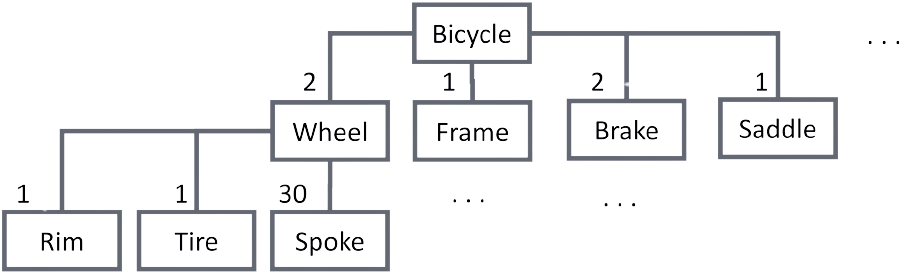
\includegraphics[width=1.0\linewidth]{images/BoM.png}
\end{figure}
The entity relationship model is the following:
\begin{figure}[H]
    \centering
    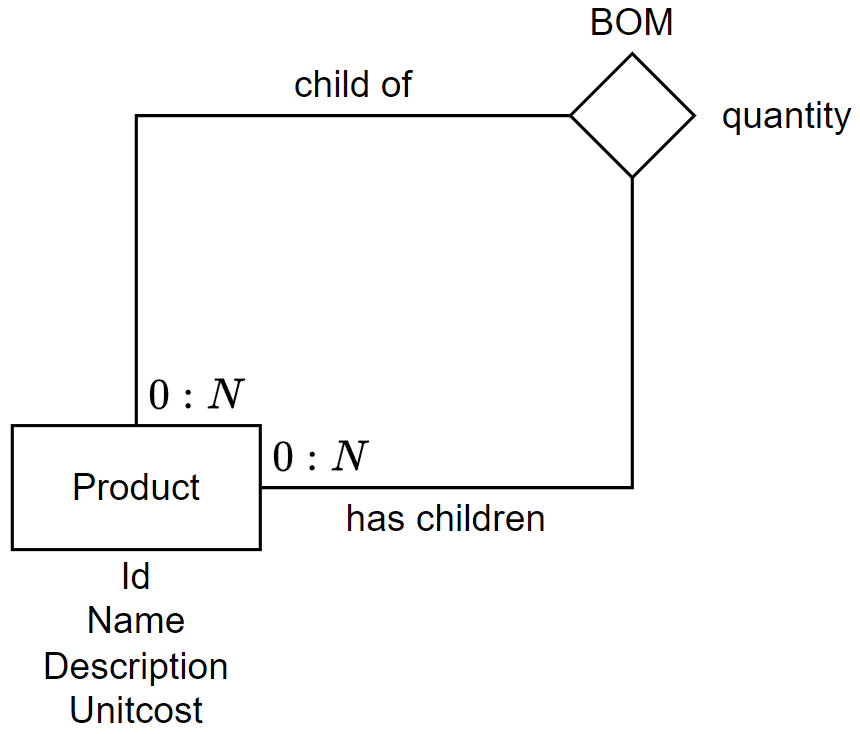
\includegraphics[width=0.5\linewidth]{images/e-r1.png}
\end{figure}
The relational schema DDL of the given database is: 
\begin{lstlisting}[style=SQL]
CREATE TABLE 'product' (
'id'            INT             NOT NULL AUTO_INCREMENT,
'unitcost'      INT             NOT NULL,
'name'          VARCHAR(45)     NOT NULL,
'description'   VARCHAR(45)     DEFAULT NULL,
PRIMARY KEY ('id')
) 
CREATE TABLE 'subparts' (
'father'        INT             NOT NULL,
'child'         INT             NOT NULL,
'quantity'      INT             NOT NULL,
PRIMARY KEY ('father','child'),
KEY 'childtoproduct_idx' ('child'),
CONSTRAINT 'childtoproduct' FOREIGN KEY ('child') REFERENCES 'product' ('id'),
CONSTRAINT 'fathertoproduct' FOREIGN KEY ('father') REFERENCES 'product' ('id')
)           
\end{lstlisting}
The relational model is: 
\begin{itemize}
    \item Product(\underline{id}, unitcost, name, description)
    \item Subparts(\underline{father}, \underline{child}, quantity)
\end{itemize}
Given the specifications, write the entity classes of the ORM mapping, including annotations for the attributes and for the relationships, fetch type of attributes and of relationships, and operation cascading policies for relationships (when not by default).

\subsection*{Solution}
Given the specifications write the entity classes of the ORM mapping, including annotations for the attributes and for the relationships, fetch type of attributes and of relationships, and operation cascading policies for relationships (when not by default). 
\begin{itemize}
    \item BoM: from father product to children product we have to use the annotations: 
        \begin{lstlisting}[style=Java]
@ManyToMany
        \end{lstlisting}
        From children product to father product we have to use these annotations: 
        \begin{lstlisting}[style=Java]
@ManyToMany
        \end{lstlisting}
        The owner of the relation is entity project. 
    \item 
\end{itemize}
The entity product is defined as:  
    \begin{lstlisting}[style=Java]
@Entity
@NamedQueries({
@NamedQuery(name = "BomProduct.findAll", query = "SELECT p FROM BomProduct p"),
@NamedQuery(name = "BomProduct.findAllTop", query = "SELECT p FROM BomProduct p WHERE p.fathers IS EMPTY") })

public class BomProduct implements Serializable {
    ...
    private static final long serialVersionUID = 1L;
    @Id @Column(name="id") @GeneratedValue(strategy = GenerationType.IDENTITY)
    private int id;
    private String description;
    private String name;
    private int unitcost;
    ...
    @ElementCollection(fetch = FetchType.EAGER)
    @CollectionTable(name = "subparts",joinColumns = @JoinColumn(name = "father"))
    @MapKeyJoinColumn(name = "child")
    @Column(name = "QUANTITY")
    private Map<BomProduct, Integer> subparts;

    @ManyToMany
    @JoinTable(name = "subparts",
            joinColumns = @JoinColumn(name = "child"),
            inverseJoinColumns = @JoinColumn(name ="father"))
    private List<BomProduct> fathers;
    ...            
}
    \end{lstlisting}
The better way is to make the many-to-many relationships with attributes a weak entity like in the following image. 
\begin{figure}[H]
    \centering
    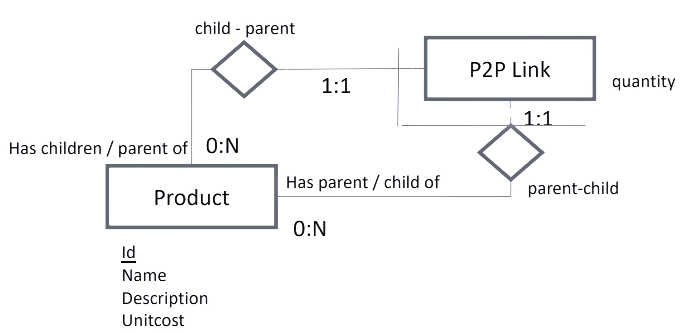
\includegraphics[width=0.5\linewidth]{images/BoMweak.png}
\end{figure}
The entity P2PLinkID is defined as:  
\begin{lstlisting}[style=Java]
@Embeddable
public class P2PLinkID implements Serializable {
    private static final long serialVersionUID = 1L;
    private int father;
    private int child;

    public P2PLinkID() { }

    public P2PLinkID(int father, int child) {
        super();
        this.father = father;
        this.child = child;
    }
    ...
}
\end{lstlisting}
The entity P2PLink is defined as:  
\begin{lstlisting}[style=Java]
@Entity
public class P2PLink implements Serializable {
    private static final long serialVersionUID = 1L;

    @EmbeddedId
    private P2PLinkID id;

    @ManyToOne
    @MapsId("father") // reference to the foreign key attribute
    @JoinColumn(name = "father")
    private BomProduct father;

    @ManyToOne
    @MapsId("child") // reference to the foreign key attribute
    @JoinColumn(name = "child")
    private BomProduct child;

    private int quantity;
    ...
}
\end{lstlisting}
The entity product is defined as:  
\begin{lstlisting}[style=Java]
@Entity
public class BomProduct implements Serializable {
    private static final long serialVersionUID = 1L;

    @Id @GeneratedValue(strategy = GenerationType.IDENTITY)
    private int id;
    private String description;
    private String name;
    private int unitcost;

    // getters setters and constructors

    @OneToMany(mappedby="father")
    private List<P2PLink> children;

    @OneToMany(mappedby="child")
    private List<P2PLink> fathers;
    ...
}
\end{lstlisting}
    \section{Exercise three}

The busy time of a virtual machine is 3 hours every 4 hours. 
Its utilization is 80\%, and on average, it is serving 5 jobs simultaneously. 
Determine:
\begin{enumerate}
    \item The system throughput.
    \item The average response time.
\end{enumerate}

\subsection*{Solution}
Given:
\[B=3\qquad T=4\qquad U=0.8 \qquad N=5\]
The utilization calculated from busy time and total time does not match the given utilization:
\[U=\dfrac{B}{T}=\dfrac{3}{4}=0.75\neq 0.8\]
The given data is inconsistent; therefore, this exercise cannot be solved.
    \section{Indices}
Search engines are designed to deliver results as quickly as possible, since any delay can impact user experience and attention. 
Responses must be returned within tenths of a second, so search engines are optimized for speed.

At the heart of this efficiency is the inverted index, which is the core data structure used by search engines to retrieve documents.

\subsection{Inverted indices}
An inverted index consists of posting lists, which map term IDs to document IDs. 
The basic idea is to create a mapping between terms and the documents that contain them, so that when a user searches for a term, the system can quickly find all the relevant documents.

To optimize for speed and reduce storage space, inverted indices often use integer compression algorithms, allowing for quick decompression and reducing the overall size of the index.

When calculating a retrieval function, the process typically involves joining posting lists. 
The documents within these lists are sorted by term frequency. 
This sorting allows for early termination of the results list computation, so irrelevant documents are discarded quickly.

\subsection{Positional indices}
In many cases, it's not just about whether a term appears in a document, but where it appears. 
To capture this, some indices maintain positional information, recording the exact locations of terms within documents. 
This allows for the calculation of proximity between query terms, which can be a useful indicator of relevance.

Moreover, the location of words within a webpage can influence their importance. 
In addition, certain statistically significant bigrams and trigrams are often identified and indexed separately. 
These are usually discovered using a technique like pointwise mutual information, which measures the association between terms. 
These bigrams or trigrams often have their own posting lists, as they can provide more context to queries.

\subsubsection{Crawlers}
To populate the index, web crawlers scour the web, following hyperlinks to discover and add new pages to the search engine's database. 
Effective crawling involves two main challenges:
\begin{itemize}
    \item \textit{Prioritizing URLs}: the crawler must decide which URLs to visit first based on factors like relevance and likelihood of finding fresh content.
    \item \textit{Re-visiting websites}: determining how often to revisit a website to check for updates is critical to ensuring that the index remains fresh and up to date.
\end{itemize}
\noindent At the scale of the web, crawlers must also be robust enough to handle different types of content, including dynamically generated pages.
Additionally, web crawlers must detect and manage duplicate content. Many different URLs may lead to the same content, and the crawler needs to ensure that it doesn't index the same page multiple times.

To manage these challenges, a distributed crawler architecture is typically used, with a centralized URL list to keep track of the pages the crawler needs to visit. 
Crawlers also respect robots.txt files, which are placed in the root directory of websites. 
These files tell crawlers which pages or sections of the site they are allowed to crawl and index, helping website owners manage how their content is indexed.
    \section{Fuzzy logic}

Fuzzy logic is an infinite-valued logic with truth values ranging from 0 to 1, where propositions are expressed in the form of "A is L," where:
\begin{itemize}
    \item $A$ is a linguistic variable.
    \item $L$ is a label representing a fuzzy set.
\end{itemize}
Formally, a linguistic variable is defined by a 5-tuple (X, T(X), U, G, M), where: 
\begin{itemize}
    \item $X$ is the name of the variable.
    \item $T(X)$ is the set of term for $X$, each corresponding to a fuzzy variable denoted by $T(X)$ and ranging on $U$.
    \item $U$ is the universe of discourse defined on a base variable $u$.
    \item $G$ is the syntactic rule used to generate the interpretation $X$ of each value $u$.
    \item $M$ is the semantic rule used to associate to $X$ its meaning.
\end{itemize}
\begin{example}
    Let's define a linguistic variable for age as follows:
    \begin{itemize}
        \item $X$ is a linguistic variable labelled "age".
        \item $\textnormal{U}=[0,100]$.
        \item $\textnormal{T(X)}=\{old, middle-aged, young, \dots\}$.
        \item $\textnormal{u}=[0,+\infty]$.
        \item $M$ represents the definition in terms of fuzzy sets for the values of $X$.
        \item $G$ is responsible for the fuzzy matching interpretation of $u$.
    \end{itemize}
\end{example}
Now that we have defined the linguistic variable, it is possible to express a simple proposition as "p: X is F", where:
\begin{itemize}
    \item $X$ is a linguistic variable.
    \item $F$ is the label of a fuzzy set defined on $U$, representing a fuzzy predicate.
    \item $\mu_{\textnormal{F(x)}}$ is the membership function defining $F$, and it is interpreted as the truth value for the proposition $p$ ($\textnormal{T(p)}=\mu_{\textnormal{F(x)}}$).
\end{itemize}
Hence, the truth value of the proposition $P$ is a fuzzy set defined on the interval $[0,1]$.
\begin{example}
    Consider the simple proposition "$p$: temperature is high", with $X$ representing temperature and $F$ representing high. 
    We can determine the truth value of this proposition using the graph of the membership function as shown below:        
    \begin{figure}[H]
        \centering
        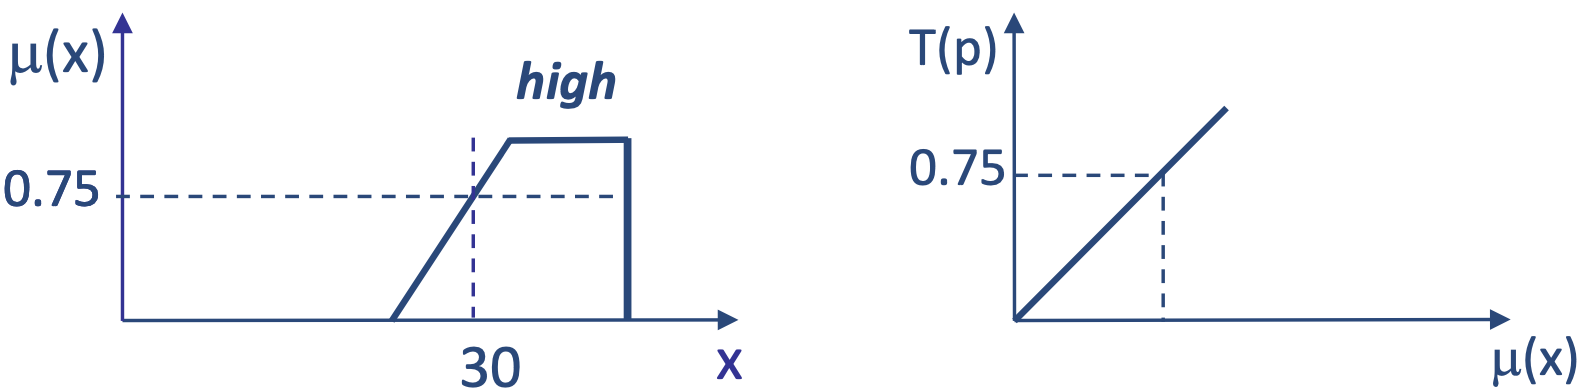
\includegraphics[width=0.5\linewidth]{images/temperature.png}
    \end{figure}
    Consequently, the truth value of the given proposition is 0.75.
\end{example}

It is also possible to express qualified, non-conditional propositions using the syntax "$p$: ($X$ is $F$) is $S$", where:
\begin{itemize}
    \item $S$ is a fuzzy truth qualifier.
    \item $F$ is a fuzzy set.
    \item $p$ is truth qualified.
\end{itemize}
\begin{example}
    Consider the conditional proposition "$p$: age of Tina is young is very true", where $X$ represents age, $F$ represents young, and $S$ represents very true. 
    To determine the truth value of this proposition, we can refer to the graph of the membership function as shown below:
    \begin{figure}[H]
        \centering
        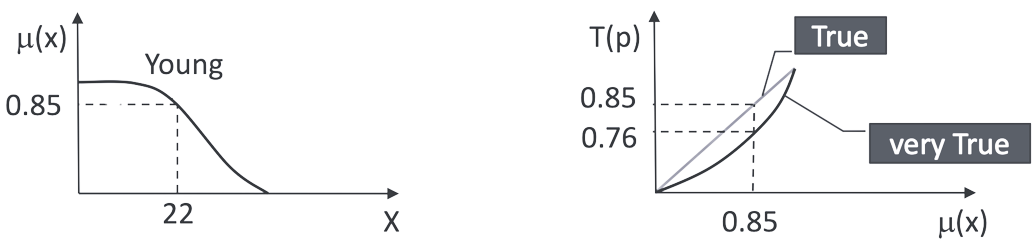
\includegraphics[width=0.5\linewidth]{images/age.png}
    \end{figure}
\end{example}

In fuzzy logic, fuzzy modifiers are employed to adjust the truth values of propositions. These modifiers can be categorized into two main types:
\begin{itemize}
    \item Strong ($m(a) \leq a \: \forall a \in [0 \dots 1]$): these modifiers strengthen the predicate, leading to a reduction in the truth value of the proposition.
    \item Weak($m(a) \geq a \: \forall a \in [0 \dots 1]$): these modifiers weaken the predicate, resulting in an increase in the truth value of the proposition.
\end{itemize}
The key properties of fuzzy modifiers include:
\begin{itemize}
    \item $m(0)=0$ and $m(1)=1$.
    \item $m$ is a continuous function. 
    \item If $m$ is a strong modifier, then $m^{-1}$ is a weak modifier, and vice versa.
    \item When combining another modifier $g$ with $m,$ and vice versa, the resulting composition is also a modifier. 
        If both $m$ and $g$ are strong (or weak), their composition is also strong (or weak).
\end{itemize}
\begin{example}
    The sentence "$x$ is young" can be represented as "($x$ is young) is true". This sentence can be modified using fuzzy modifiers in the following ways:
    \begin{itemize}
        \item $x$ is very young is true.
        \item $x$ is young is very true.
        \item $x$ is very young is very true.
    \end{itemize}
    Graphically, we can visualize the modified membership function as follows:
    \begin{figure}[H]
        \centering
        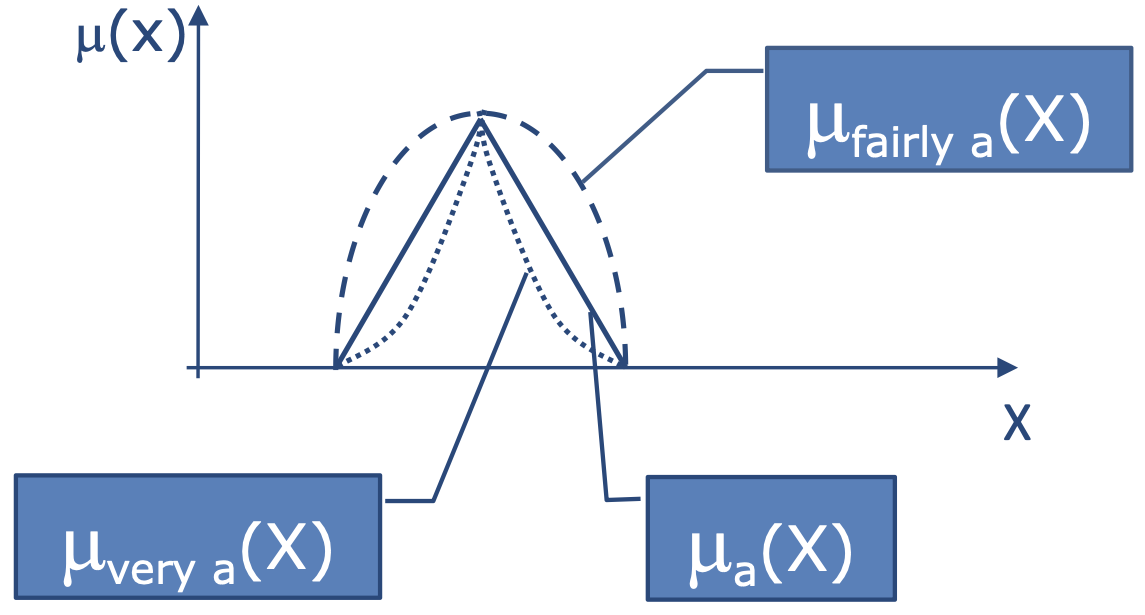
\includegraphics[width=0.3\linewidth]{images/modifiers.png}
    \end{figure}
    Here, we have:
    \begin{itemize}
        \item $\mu_{\text{very}}(x)=\mu_a(x)^2$.
        \item $\mu_{\text{fairly}}(x)=\mu_a(x)^{\dfrac{1}{2}}$.
    \end{itemize}
\end{example}
    \section{Traveling salesman problem}

Given a directed graph $G=(N,A)$ with cost $c_{ij} \in \mathbb{Z}$ for each are $(i,j) \in A$, determine a circuit of minimum total cost visiting every node exactly once. 
\begin{definition}[\textit{Hamiltonian circuit}]
    A Hamiltonian circuit $C$ of $G$ is a circuit that visits every node exactly once. 
\end{definition}
Therefore, by representing $H$ as the set encompassing all Hamiltonian circuits within graph $G$, the problem can be formulated as:
\[\min_{C \in H}{\sum_{(i,j) \in C}{c_{ij}}}\]
It's important to note that this problem is classified as $\mathcal{N}\mathcal{P}$-hard. 
    \section{Localization}

\subsection{Preprocessing}
in general, normalization is useful in gradient-based optimizers.
Normalization is meant tobring training data “around the origin” and
possibly further rescale the data
in practice, optimization on pre-processed data is made easier and
results are less sensitive to perturbations in the parameters
There are several options: 
\begin{itemize}
    \item PCA — based preprocessing: this is performed after having «zero-centered» the data
    \item mean subtraction
    PCA/Whitening preprocessing are not commonly used with CNN
    The most frequent option is to zero-center the data, and it is common
    to normalize every pixel as well
\end{itemize}
Normalization statistics are parameters ofyour ML model: Any
preprocessing statistics (e.g. the data mean) must be computed on
training data, and applied to the validation test data.
Do not normalize first and then split in training, validation, test
When asing pretrained model, remember to import (and use!) their
pre-processing functions

\subsection{Batch normalization}
Considera batch of activations $\{x_i\}$, the following transformation bring these to unit variance and zero mean: 
\[x_i^\prime=\dfrac{x_i-\mathbb{E}[x_i]}{\sqrt{\text{Var}[x_i]}}\]
Here, $\mathbb{E}[x_i]$ and $\text{Var}[x_i]$ are computed from each batch and separately for each channel
a furthera parametric transformation
\[y_{i,j}=\gamma_jx_i^\prime+\beta_j\]
Here, the parameters $\gamma$ and $\beta$ are learnable scale and shift parameters. 
We have $\gamma$ and $\beta$ for each channel of the input activation. 
The expected value and variance are non trainable parameters. 

During testing batch normalization becomesa linear operator! Can be
fused with the previous fully-connected or conv layer.
in practice networks that use Batch Normalization are significantly more
robust to bad initialization.
Typically Batch Normalization is ased in between FC layers of deep CNN,
but sometimes also between Conv Layers.

Pros:
Makes deep networks much easier to train!
improves gradient flow
Allows higher learning rates, faster convergence
Networks become more robast to initialization
Acts as regularization during training
Zero overhead at test-time: can be fused with conv!
Watch out:
Behaves differently during training and testing: this isa very
common source of bugs!

\subsection{Bounding box estimation}
The inpat image containsa single relevant object to be classified ina
fixed set of categories
The tasks are:
1) assign the object class to the image
2) locate the object in the image by its bounding box
A training set of annotated images with label and
a bounding box around each object is required
Extended localization problems involve regression over
more complicated geometries (e.g. human skeleton)ù

Assign to an input image $I\in \mathbb{R}^{R\times C \times 3}$ the coordinates $(x,y, h, w)$ of the bounding box enclosing the object
\[I\rightarrow(x,y, h, w)\]
Sim lest So ution
Traina regression network to predict the bounding box


\subsection{Localization}
Assign to an input image $I\in \mathbb{R}^{R\times C \times 3}$ a labelf froma fixed set of categories $\Lambda$ the coordinates $(x,y, h, w)$ of the bounding box enclosing the object
\[I\rightarrow(x,y, h, w)\]
This isa multi-task learning problem, as the two outputs have
different nature
Traina network to predict both the class label and the bounding box
The training loss has to bea single scalar since we compute gradient
a scalar function with respect to network parameters.
Minimizea multitask loss to merge two losses:
\[\mathcal{L}(x)=\alpha\mathcal{S}(x)+(1-\alpha)\mathcal{R}(x)\]
Here, $\alpha\in[0,1]$ is an hyper parameter ofthe network.
Watch outthat $\alpha$ directly influences the loss definition, tuning might be
difficult. Better to do cross-validation looking at some other loss (loss
value for different values of might be meaningless).
it is also possible to adopta pre-trained model and then train the two
FC separately... however it is always better to perform at least some
fine taning to train the two jointly.
However, this solution is not:
Able to handle multi-class classification
Predict bounding boxes outside the image
To implementa multi-task loss it is necessary to modify the training loop

\subsection{Human pose estimation}
Pose estimation is formulated asa CNN-regression problem towards body
joints. This isa localization task. 

The network receives as input the whole image, capturing the fullcontext of each body joints.
The approach is very simple to design and train. Training problems can
be alleviated by transfer learning of existing classification networks
Pose is defined asa vector of $k$ joints location for the human body,
possibly normalized w.r.t. the bounding box enclosing the human.
Traina CNN to predicta vector  $2k$ as oatpat by using an Alexnet-like
architecture.
Adopta regression loss of the estimated pose parameters over the
annotations.
• The network always providea fixed whena fewjoints are not visible.
Redace overlitting by augmentation (translation and flips).
Multiple networks have been trained to improve localization by refining
joint position ina crop around the initial detection.


\subsection{Saliency maps and weakly supervised localization}
In supervised learninga model \mathcal{M} performing inference in $Y$
\[\mathcal{M}:X\rightarrow Y\]
Requires a training set $\text{TR}\subset X \times Y$, namely training couples are of the same type as classifier input-output.
For some tasks (e.g. segmentation) these type ofannotations are very expensive to gateher.

In weak supervision we obtain a model able to solvea task in $Y$, but asing labels that are easier to gather ina different domain $K$. Therefore, $\mathcal{M}$ after training perform inference as
\[\mathcal{M}:X \rightarrow Y\]
but it is trained using $\text{TR}\subset X \times K$, where $K \neq Y$. 

\paragraph*{Weakly supervised localization}
Perform a localization $\mathcal{M}:X\rightarrow\mathbf{R}^4$ without images training images annotated bounding box.
The training set is typically annotated for classification, thus $\text{TR}\subset X \times \Lambda$ with image-label pairs $\{(I,\ell)\}$ whith no localization information provided.
Basically, yoa traina classifier and you get also localization estimates.

\paragraph*{GAP revisited}
The advantages ofGAP layer extend beyond simply acting asa structural
regalarizer that prevents overfitting (as shown in the NiN paper)
in fact, CNNs canretaina remarkable localization ability until the final
layer. Bya simple tweak it is possible to easily identify the discriminative
image regions leading toa prediction.
A CNR traineb ono*i•
cl categorization is success/u//y able to localize the
biscriminative regions |or action cIassi|ication as the objects that the
humans areinteracting w/t// rather than thehumans themselves

\paragraph*{Class Activation apping}
Identifying exactly which regions of an image arebeing used for
discrimination.
CAm needs a classifier trained with a GAP layer, FC layer after the GAP and a minor tweak to obtain saliency maps. 

\paragraph*{The GAP layer}
Assume yoa have traineda CNN
architecture having atthe end ofthe
convolutional block: $n$ feature maps $f_k(\cdot,\cdot)$ having
resolution “similar” to the inpat
image and a GAP layer that competes $n$ averages $F_k,k=1,\dots,n$. 
Add (and train)a single FC layer after the GAP.
The FC computes $S_c$ for each class $c$ as the weighted sum of $\{F_k\}$, where weights are defined during training.
Then the class probability $\Pr_c$ via softmax. 
Wehn computing
\[S_c\sum_{k}w_k^cF_k\]
Here, $w^c_k$ encodes the importance of $F_k$ for the class $c$, $\{w_k^c\}_{k,c}$ are all the parameters of the last FC layer. 
Perpective change in core interpretation
\[S_c=\sum_kw_k^c\sum_{x,y}f_k(x,y)=\sum_{x,y}\sum_kw_k^cf_k(x,y)\]
And CAM is defined as
\[M_c(x,y)=\sum_kw_k^cf_k(x,y)\]
Here, $M_c(x,y)$ directly indicates the importance of the activations ar $(x,y)$ for predicting the class $c$. 
Last layer weights $\{w_k^c\}$ encode how relevant each feature map is to yield the final prediction.

\paragraph*{Remarks}
CAM canbeincluded in any pre-trained network, as long as all the FC
layers at the end are removed
The FC ased forCAM is simple, few neurons and no hidden layers
Classification performance might drop (in VCC removing FC means
loosing go'/o of parameters)
CAM resolution (localization accuracy) can improve by «anticipating»
GAP to larger convolutional feature maps (bat this reduces the
semantic information within these layers)
GAP: encourages the identification of the whole object, as all the parts
of the values in the activation map concurs to the classification
GMP (Global Max Pooling): it is enough tohavea high maximum, thas
promotes specific discriminative features
















\subsection{CNN visualization}
For the first layer we can quite easily extract the filter. 

The first layer seems tomatch low-level features such as edges
and simple patterns that
are discriminative to describe the data

Difficult to interpret deeper layers

Another way to determine «what thedeepest layer see» is
required

We can do the following: 
1. Selecta neuron ina deep layer ofa pretrained CNN onl mageNet
2. Perform inference and store the activations
for each input image.
z. Select the image yielding the maximum
activation.
4. Showtheregions (patches) corresponding to
the receptive field of the neuron.
5. Iterate for many neurons.



Computing Images maximally activating softmax neuron
Adopt gradient descent to maximally activatea neuron before the
softmax, thus the network «score»: the higher the most likely the
network predicts that class
\[\hat{I}=\argmax_I S_c(I)+\lambda{\left\lVert I\right\rVert}_2^2 \]
Here $\lambda> 0$ regularization parameter, $c$ isa given oatpat class.
To improve the smoothness ofacquired imags is necessary to adda
regularization term
Maximize this function through gradient ascent over the network inpat.
Repeat this operation for neurons corresponding to different classes $c$. 



\subsection{Explanations}
Deep Neural Networks have
Million parameters: their inner
functioning is totally obscure.
Healthy scepticism to resort to NN
decision in critical tasks (e.g.
medical domain) oreven services
(e.g., blocking credit cards).
Vivid research activity around
gaining an understanding of
Neural Network decision.
Saliency aps to nderstan Model istakes
Saliency aps to Discover Systematic rrors
We may use Grand CAM and CAM based tecniques
    \section{Probabilistic model checking}

Many systems operate in environments influenced by randomness, making it difficult to guarantee absolute correctness.
Instead of relying solely on nondeterminism, we often seek probabilistic guarantees.
To analyze such scenarios, we extend traditional models to include probabilities, utilizing structures like Markov chains and Markov Decision Processes. 
This allows for verifying properties such as:
\begin{itemize}
    \item \textit{Qualitative properties}: ensuring that a good event happens with probability 1, or that a bad event has probability 0.
    \item \textit{Quantitative properties}: checking if a desired event occurs with at least 95\% probability, or if an undesired event happens with less than 5\% probability.
\end{itemize}

\subsection{Markov chains}
Markov chains are widely used to evaluate the performance and reliability of information-processing systems. 
They extend traditional transition systems by associating probabilities with state transitions rather than relying on nondeterministic choices.
\begin{definition}[\textit{Discrete time Markov chain}]
    A discrete time Markov chain $\mathcal{M}$ is defined as a tuple $\mathcal{M}=\left\langle S,\Pr,\ell_{\text{init}},\text{AP},L\right\rangle$ where: 
    \begin{itemize}
        \item $S$ is a countable, nonempty set of states.
        \item $\Pr : S \times S \rightarrow [0, 1]$ defines transition probabilities, ensuring that for every state $s$: $\sum_{s^\prime\in S}\Pr(s,s^\prime)=1$. 
        \item $\ell_{\text{init}}:S\rightarrow [0,1]$ is the initial probability distribution, such that $\sum_{s\in S}\ell_{\text{init}}(s)=1$.
        \item $\text{AP}$ is a set of atomic propositions.
        \item $L : S \rightarrow 2^{\text{AP}}$ labels each state with relevant propositions.
    \end{itemize}
\end{definition}
\noindent Since discrete time Markov chains lack nondeterminism, they cannot model interleaving behavior in concurrent systems.

\subsubsection{Probabilistic logic for Markov chains}
Unlike traditional model-checking techniques, where infinite paths might lead to unrealistic behaviors, probability-based logics help us analyze realistic system behaviors.

Given a linear time logic formula $\phi$, the probability of $\phi$ holding in state $s$ is:
\[\Pr(s\models\phi)=\Pr_s\left\{\pi\in\text{paths}(s)\mid\pi\models\phi\right\}\]
Here, $\Pr_s$ is the total probability of all paths starting at $s$ where $\phi$ holds.

\subsection{Probabilistic Computation Tree Logic}
Probabilistic Computation Tree Logic extends Computation Tree Logic by incorporating probability bounds, allowing for the formal verification of probabilistic systems.

\subsubsection{Syntax}
The syntax of Probabilistic Computation Tree Logic consists of state and path formulae. 
State formulae describe properties of individual states:
\[\Phi::=\text{true}\mid a\mid \Phi_1\land\Phi_2\mid\lnot\Phi\mid\mathbb{P}_J(\phi)\]
\noindent Here, $a \in AP$ is an atomic proposition, $\phi$ is a path formula, and $J \subseteq [0, 1]$ is a probability interval.

Path formulae define properties over execution paths:
\[\phi::=\bigcirc\Phi\mid\Phi_1\cup\Phi_2\mid\Phi_1\cup^{\leq n}\Phi_2\]
\noindent Here, $\bigcirc$ represents the next operator, $\cup$ denotes the until operator, and $\cup^{\leq n}$ expresses bounded until with a maximum of $n$ steps.

\subsubsection{Semantic}
Probabilistic Computation Tree Logic is interpreted over a Markov chain, where the semantics of the non-probabilistic fragment follow those of Computation Tree Logic. 
The probability operator is defined as:
\[s\models\mathbb{P}_j(\phi)\Leftrightarrow\Pr(s\models\phi)\in J\]
Here, $\Pr(s\models\phi)$ represents the probability that paths originating from state $s$ satisfy $\phi$. 
The following rules define how Probabilistic Computation Tree Logic formulas are evaluated:
\begin{itemize}
    \item $s \models a \Leftrightarrow a \in L(s)$
    \item $s \models \lnot\Phi \Leftrightarrow s \not\models \Phi$
    \item $s \models \Phi \land \psi \Leftrightarrow s \models \Phi \land s \models \psi$
    \item $\pi \models \bigcirc \Phi \Leftrightarrow \pi[1] \models \Phi$
    \item $\pi \models \Phi \cup \psi \Leftrightarrow \exists j \geq 0 \quad(\pi[j] \models \psi \land (\forall 0 \leq k < j. \pi[k] \models \Phi))$
    \item $\pi \models \Phi \cup^{\leq n} \psi \Leftrightarrow \exists 0 \leq j \leq n \quad(\pi[j] \models \psi \land (\forall 0 \leq k < j. \pi[k] \models \Phi))$
\end{itemize}
Here, for a path $\pi = s_0 s_1 s_2 \dots$ and $\pi[i]$ denotes the $(i+1)$-th state of $\pi$.

\subsubsection{Model checking}
The Probabilistic Computation Tree Logic model checking problem involves determining if a given state in a Markov chain satisfies a Probabilistic Computation Tree Logic formula. 
Given a finite Markov chain $\mathcal{M}$, a state $s$ in $\mathcal{M}$, and a Probabilistic Computation Tree Logic state formula $\Phi$, the problem is to determine whether $s \models \Phi$.
This is achieved by computing the satisfaction set $\text{sat}(\Phi)$ using a bottom-up traversal of the formula's parse tree
\begin{theorem}
    For finite Markov chain $\mathcal{M}$ and Probabilistic Computation Tree Logic formula $\Phi$, the model checking problem $\mathcal{M} \models \Phi$ can be solved in time: 
    \[\mathcal{O}\left(\text{poly}\left(\text{size}\left(\mathcal{M}\right)\cdot n_{\max}\cdot\left\lvert \Phi\right\rvert\right)\right)\]
    Here, $n_{\max}$ is the maximal step bound appearing in a bounded until subformula $\Psi_1\cup^{\leq n}\Psi_2$ of $\Phi$, and $n_{\max}=1$ if $\Phi$ contains no bounded until operators.
\end{theorem}
Restricting probability bounds to greater than zero, equal to one, equal to zero or less than one results in a qualitative fragment of Probabilistic Computation Tree Logic, which allows reasoning without explicit probability values and improves model checking efficiency.
\begin{property}
    There is no Computation Tree Logic formula that is equivalent to $\mathbb{P}_{=1}(\Diamond a)$.
\end{property}
\begin{property}
    There is no Computation Tree Logic formula that is equivalent to $\mathbb{P}_{>0}(\square a)$.
\end{property}
\begin{property}
    There is no qualitative Probabilistic Computation Tree Logic formula that is equivalent to $\forall\Diamond a$. 
\end{property}
\begin{property}
    There is no qualitative Probabilistic Computation Tree Logic formula that is equivalent to $\exists\square a$.
\end{property}

\subsection{Markov decision processes}
A Markov Decision Process extends Markov chains by introducing nondeterminism, making them useful for modeling concurrent systems.
\begin{theorem}
    For a finite A Markov Decision Process $\mathcal{M}$ and a Probabilistic Computation Tree Logic formula $\Phi$, the model checking problem $\mathcal{M} \models \Phi$ can be solved in time:
       \[\mathcal{O}\left(\text{poly}\left(\text{size}\left(\mathcal{M}\right)\cdot n_{\max}\cdot\left\lvert \Phi\right\rvert\right)\right)\]
    Here, $n_{\max}$ is the maximal step bound appearing in a bounded until subformula $\Psi_1\cup^{\leq n}\Psi_2$ of $\Phi$, and $n_{\max}=1$ if $\Phi$ contains no bounded until operators.
\end{theorem}

    \chapter{Properties}
    \section{Exercise one}

Consider the C program below, which is affected by a typical buffer overflow vulnerability.
\begin{verbnobox}[\verbarg]
#include <stdio.h>
#include <stdlib.h>
#include <string.h>

void vuln() {
    char buf[32];

    scanf("%s", buf);
    if (strncmp(buf, "Knight_King!", 12) != 0) {
        abort();
    }
}

int main(int argc, char** argv) {
    vuln();
}
\end{verbnobox}
\begin{enumerate}
    \item Assume that the program runs on the usual IA-32 architecture (32-bits), with the usual \texttt{cdecl} calling convention. 
        Also assume that the program is compiled without any mitigation against exploitation (ASLR is off, stack is executable, and stack canary is not present).
        Draw the stack layout when the program is executing the instruction at line seven, showing:
        \begin{itemize}
            \item Direction of growth and high-low addresses.
            \item The name of each allocated variable.
            \item The boundaries of frame of the function frames (\texttt{main} and \texttt{vuln}).
        \end{itemize}
        Show also the content of the caller frame.
    \item Write an exploit for the buffer overflow vulnerability in the above program. 
        Your exploit should execute the following simple shell code, composed only by four instructions: \texttt{0x12 0x34 0x56 0x78}.
        Write clearly all the steps and assumptions you need for the exploitation, and show the stack layout right after the execution of the \texttt{scanf()} during the program exploitation.
\end{enumerate}

\subsection*{Solution}
\begin{enumerate}
    \item To represent the stack layout described, we need to allocate space for the \texttt{buf} array, the saved EBP, and the saved EIP:
        \begin{figure}[H]
            \centering
            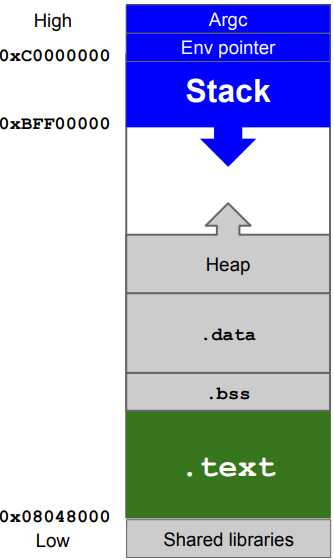
\includegraphics[width=0.5\linewidth]{images/stack.png}
        \end{figure}
    \item The stack in this case is: 
        \begin{figure}[H]
            \centering
            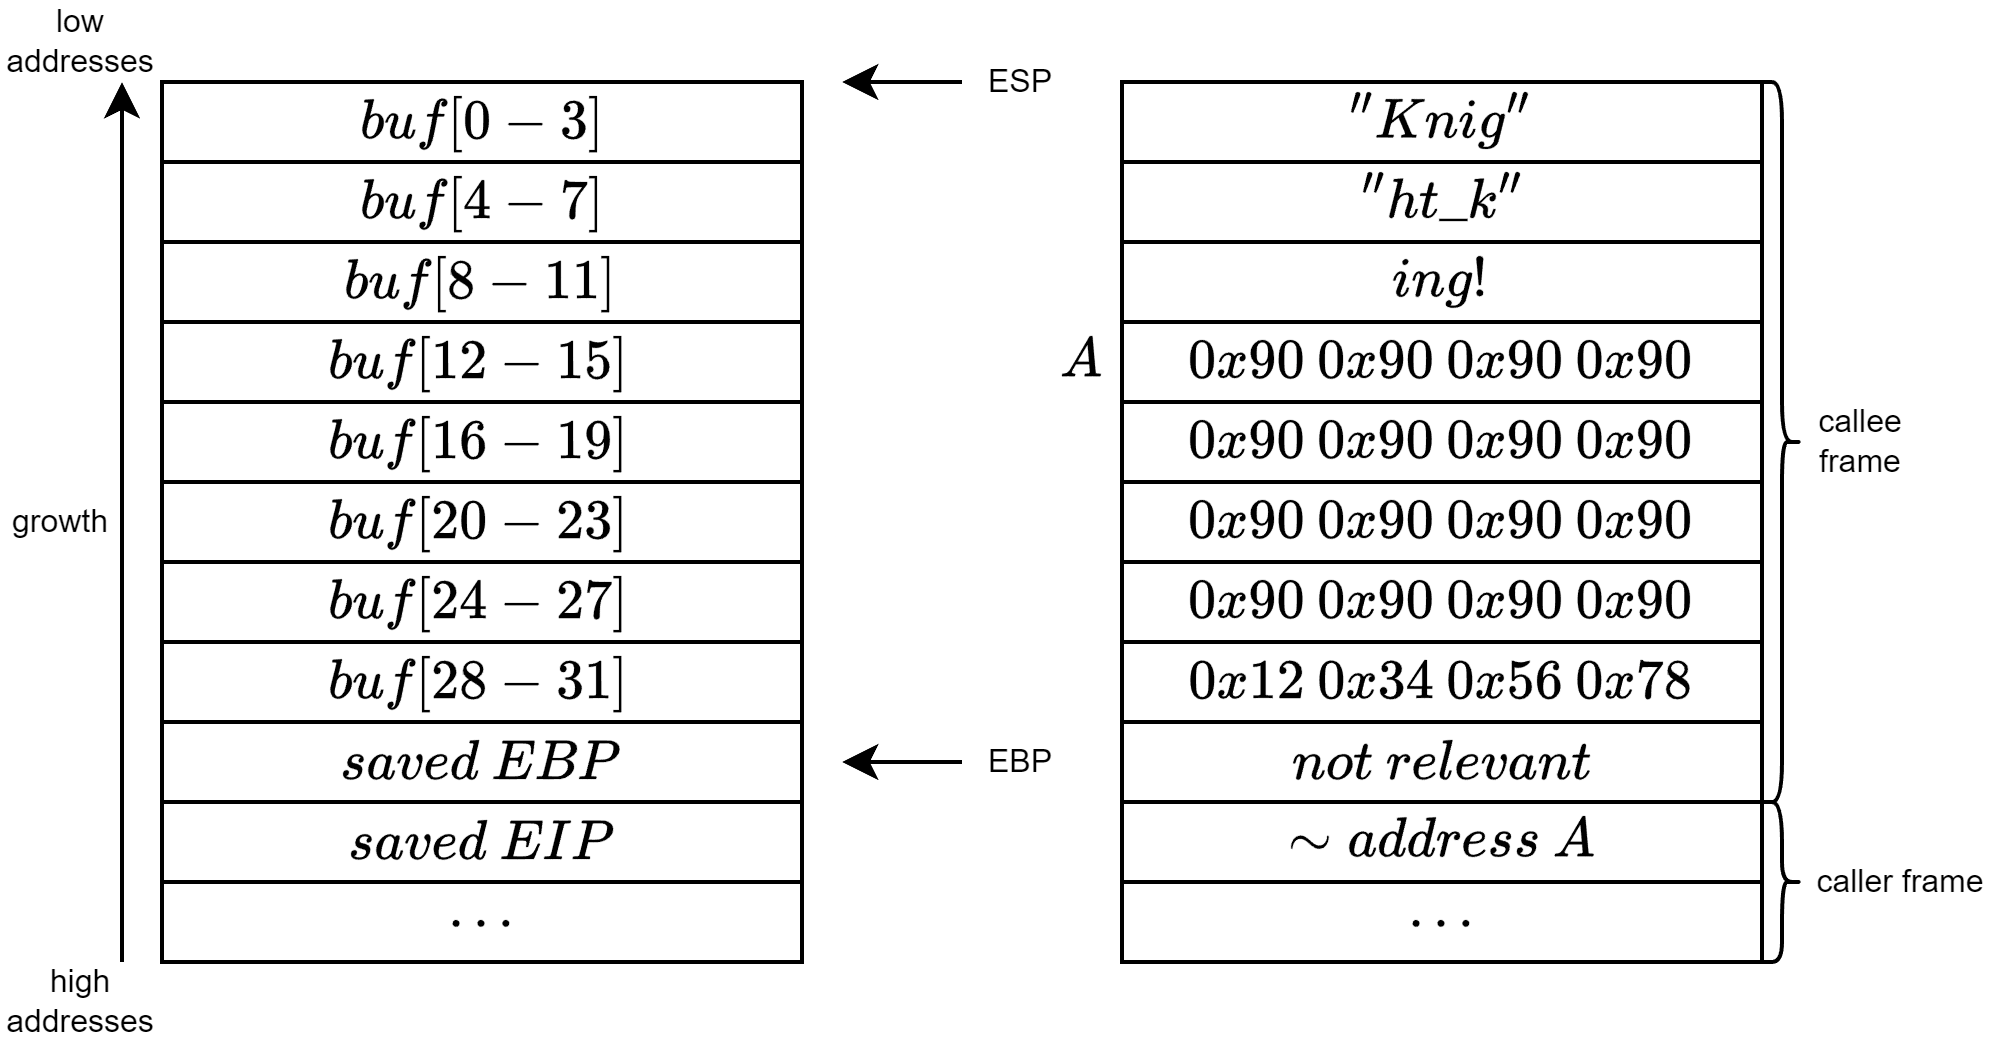
\includegraphics[width=0.75\linewidth]{images/stack1.png}
        \end{figure}
        In this layout:
        \begin{itemize}
            \item The first 16 bytes (four cells) are filled with no-operation instructions to avoid any unintended actions.
            The next 8 bytes (two cells) are reserved for the \texttt{buf} array.
            The following 4 bytes (one cell) are allocated for the saved EBP.
            The last 4 bytes (one cell) contain the address of the shell code.
        \end{itemize}
        The first twelve characters of \texttt{buf} are ensured to be different from "Knight\_King!" to avoid invoking \texttt{abort()}.
\end{enumerate}
    \section{Dependability principles}

Dependability is a critical consideration both during the design phase and during runtime operations.
During the design phase, it is essential to:
\begin{itemize}
    \item Analyze the system under development.
    \item Evaluate and measure its dependability properties.
    \item Make necessary modifications to the design as needed.
\end{itemize}
During runtime, the focus shifts to:
\begin{itemize}
    \item Detecting any malfunctions or failures that occur.
    \item Investigating and understanding the root causes of these issues.
    \item Taking appropriate reactive measures to address and mitigate the impact of the malfunctions.
\end{itemize}
Failures are commonplace in both the development and operational stages: while those in development should be averted, operational failures, being unavoidable due to the nature of system components, must be managed effectively. 
Design processes should factor in these potential failures to ensure that control and safety measures remain intact even when failures arise. 
Moreover, the effects of these failures should be predictable and deterministic rather than catastrophic.

Once upon a time, dependability was primarily a concern in safety-critical and mission-critical application domains like space exploration, nuclear facilities, and avionics. 
This was largely due to the significant cost associated with ensuring dependability, which was deemed acceptable only when absolutely necessary.
In non-critical systems, operational failures can lead to economic losses and damage to reputation, as seen in consumer products. 
However, in mission-critical systems such as satellites, automatic weather stations, surveillance drones, and unmanned vehicles, operational failures can result in serious or irreversible consequences for the mission at hand.
Safety-critical systems, on the other hand, pose a direct threat to human life if they fail during operation.
Examples include aircraft control systems, medical instrumentation, railway signaling, and nuclear reactor control systems.

    \chapter{Timed automata and languages}
    \section{Introduction}

\begin{definition}[\textit{Integer linear programming problem}]
    An Integer linear programming (ILP) problem is an optimization problem of the form:
    \begin{align*}
        \min                      \:&\: c^Tx           \\
        \textnormal{such that }     &\: Ax = b         \\
                                    &\: x \in \mathbb{Z}^n
    \end{align*}  
\end{definition}
Additionally:
\begin{itemize}
  \item If $x_j \in \left\{ 0, 1 \right\} \: \forall, j$, the problem is called binary linear programming.
  \item If $\exists, i \text{ such that }x_i \notin \mathbb{Z}^n$, then the problem is called mixed integer linear programming.
\end{itemize}
Note that the integrality condition $x_i \in \mathbb{Z}$ is non-linear, as it can be expressed as $\sin(\pi x_j)=0$.
\begin{definition}[\textit{Linear relaxation}]
    Let $ILP$ be an ILP problem:
    \begin{align*}
        z_{ILP}:=\min                      \:&\: c^Tx           \\
        \textnormal{such that }     &\: Ax \leq b               \\
                                    &\: x \in \mathbb{Z}^n      \\
                                    &\: x \leq 0
    \end{align*}  
    Then the Linear Programming (LP) problem:
    \begin{align*}
        z_{LP}:=\max                      \:&\: c^Tx                    \\
        \textnormal{such that }             &\: Ax \leq b               \\
                                            &\: x \leq 0
    \end{align*}  
    is the linear (or continuous) relaxation of $ILP$.
\end{definition}
\begin{property}[Bounds of ILP solutions]  
    For any ILP with $\max$, the optimal solution is bounded by the optimal solution of the LP relaxation:
    \[ z_{ILP} \leq z_{LP} \]
  
    For any ILP with $\min$, the optimal solution is bounded by the optimal solution of the LP relaxation:
    \[ z_{ILP} \geq z_{LP} \]
\end{property}
The feasible region of any ILP is a lattice of points, either finite or infinite, depending on the type of problem.
By removing the integrality constraint, the ILP problem becomes an LP problem, and the optimal solution of the ILP problem isn't always the optimal solution of the LP problem.
\begin{figure}[H]
    \centering
    \begin{subfigure}[b]{0.495\textwidth}
        \centering
        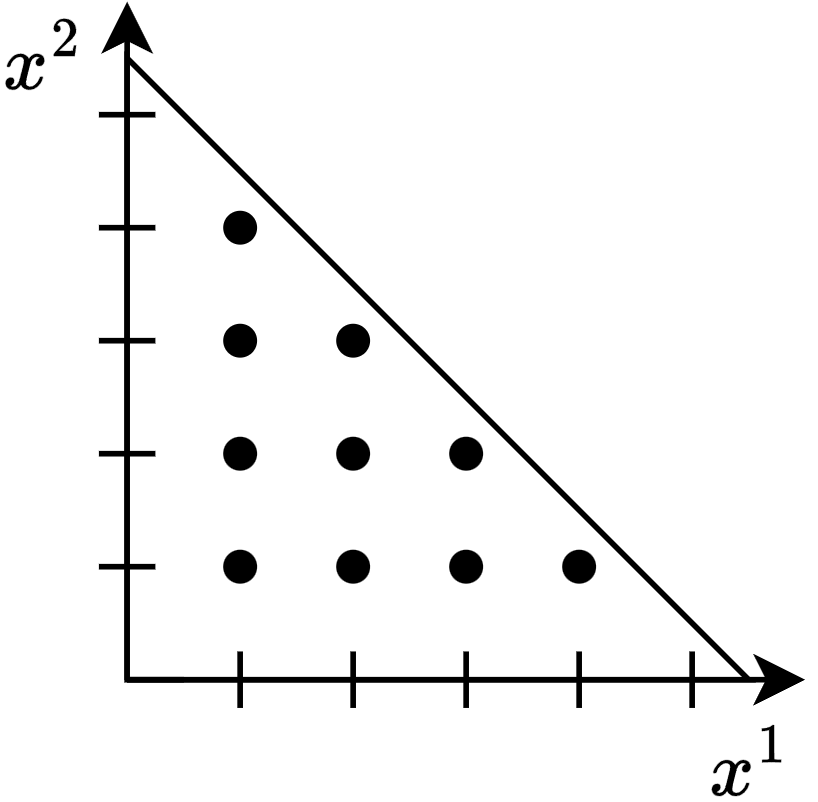
\includegraphics[width=0.4\linewidth]{images/ilp.png}
        \caption{Lattice of integer points}
    \end{subfigure}
    \begin{subfigure}[b]{0.495\textwidth}
        \centering
        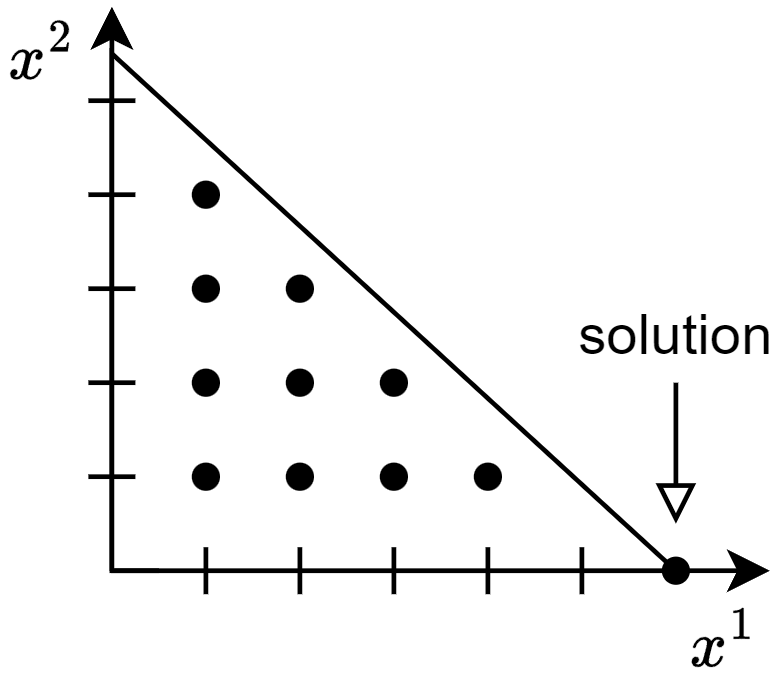
\includegraphics[width=0.4\linewidth]{images/ilp1.png}
        \caption{Relaxed lattice of integer points}
    \end{subfigure}
    \caption{Lattice of integer points}
\end{figure}
  
\subsection{Solutions of the ILP problem}
A viable approach to finding a solution to the ILP problem is to identify a solution to the LP problem and then round it to the nearest integer point.
If an optimal solution of the LP problem is an integer, it is also an optimal solution of the ILP problem. 
However, often the rounded optimal solutions of the LP are either:
\begin{itemize}
    \item \textit{Infeasible} solutions for the ILP.
    \item \textit{Useless} solutions for the ILP, as they are very different from an optimal solution of the ILP.
\end{itemize}
\begin{figure}[H]
    \centering
    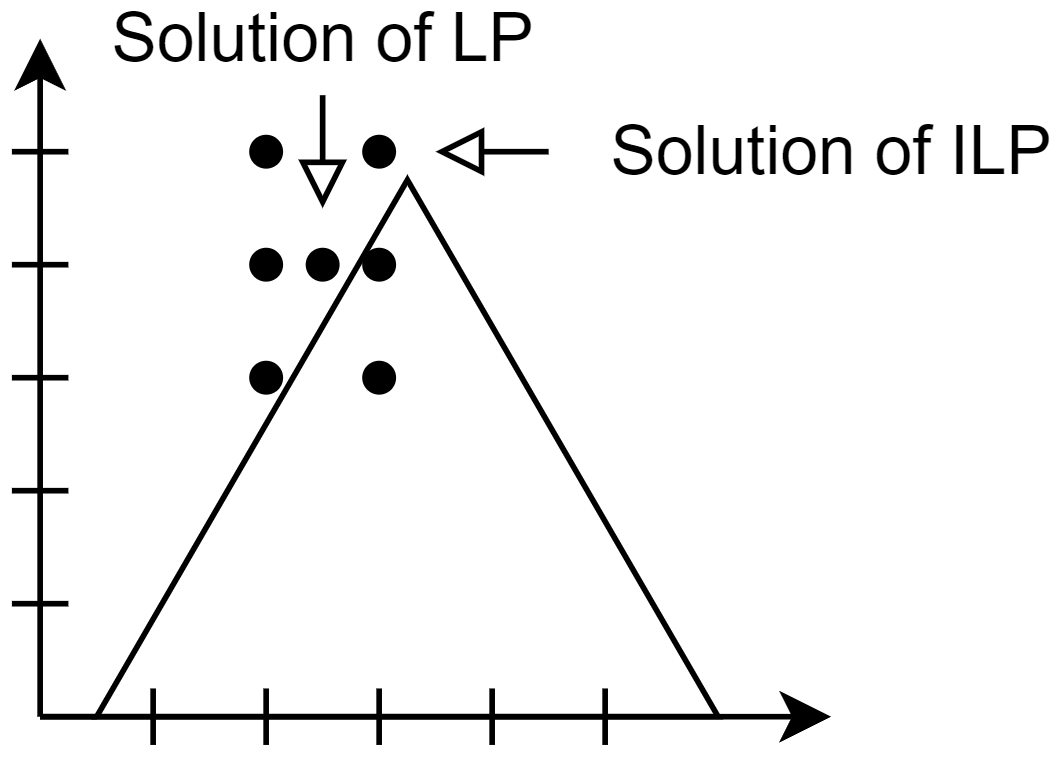
\includegraphics[width=0.25\linewidth]{images/ilp2.png}
    \caption{Solution of the LP relaxation of the ILP problem}
\end{figure}

\subsection{Solution of assignment and transportation problems}
Two crucial ILP problems, namely the assignment and transportation problems, have a solution that is the optimal solution of the LP relaxation.

\paragraph*{Assignment problem}
Given:
\begin{itemize}
    \item $m$ machines, $i = 1, \dots, m$
    \item $n$ jobs, $j = 1, \dots, n$, $n < m$
    \item $c_{ij}$ cost of assigning job $j$ to machine $i$
\end{itemize}
The goal is to determine an assignment of jobs to the machines to minimize the total cost. 
Each job must be assigned to exactly one machine, and each machine should have at least one job. 
The binary variables $x_{ij}$ represent the assignment, where:
\[ x_{ij} = 
\begin{cases}
    1 \quad & \text{if job } j \text{ is assigned to machine } i \\
    0 \quad & \text{otherwise}
\end{cases} \]
The assignment problem can be formulated as the following ILP problem:
\begin{align*}
\min        & \quad \sum_{i=1}^m \sum_{j=1}^n c_{ij} x_{ij}                                                      \\
\text{s.t.} & \quad \sum_{i=1}^{m} x_{ij} = 1 \quad \forall \, j \quad \text{at most one machine for each job}   \\
            & \quad \sum_{j=1}^{n} x_{ij} = 1 \quad \forall \, i  \quad \text{at least one job for each machine} \\
            & \quad x_{ij} \in \left\{ 0, 1 \right\} \quad \forall \, i, j
\end{align*}

\paragraph*{Transportation problem}
Given:
\begin{itemize}
\item $m$ productions plant, $i = 1, \dots, m$.
\item $n$ clients, $j = 1, \dots, n$, $n > m$ by assumption.
\item $c_{ij}$ cost of shipping one unit from plant $i$ to client $j$.
\item $p_i$ production capacity of plant $i$.
\item $d_j$ demand of client $j$.
\item $q_{ij} \geq 0$ quantity shipped from plant $i$ to client $j$.
\end{itemize}
The goal is to determine a transportation plan that minimizes the total costs while satisfying the production and demand constraints. 
The assumption is $\sum_{i=1}^m p_i \geq \sum_{j=1}^{n} d_j$.
Variables $x_{ij}$ represent the quantity shipped from plant $i$ to client $j$.

\paragraph*{Problems analysis}
In the assignment problem example, a forcing constraint is present, while the transportation problem introduces a constraint limiting the active number of variables.
\begin{definition}[\textit{Forcing constraint}]
    A constraint in the form: 
    \[ \displaystyle x \leq y\]
    is termed a forcing constraint if both $x$ and $y$ are binary variables.
\end{definition}
\begin{definition}[\textit{Constraint on binary variables}]
    A constraint of the form:
    \[ \displaystyle \sum_{i=1}^n x_i \leq 1 \]
    where all $x_i$ are binary variables, implies that at most one of the variables $x_i$ can be one. 
    Similarly, a constraint in the form: 
    \[ \displaystyle \sum_{i=1}^n x_i = 1 \]
    where all $x_i$ are binary variables, implies that exactly one variable $x_i$ must be one.
\end{definition}
The transportation problem illustrates that the optimal solution of the LP relaxation of the transportation problem is also the optimal solution of the ILP problem.
\begin{theorem}[Solution of the transportation problem]
    If in a transportation problem $p_i, \ d_{ij}, \ q_{ij}$ are all integers, all the basic feasible solutions (vertices) of its linear relaxation are integers.
\end{theorem}
\begin{proof}
    Let $A$ be an integer constraint matrix of size $\left( mn + n + m \right) \times \left( mn \right)$, where $a_{ij} \in \left\{ -1, 0, 1 \right\}$.
    The right-hand side vector $b$ is composed of integer elements.
    The optimal solution for the linear relaxation is:
    \[ x^\ast = \begin{bmatrix}
        B^{-1} b \\ 0
    \end{bmatrix}
    \qquad
    B^{-1} = \dfrac{1}{|B|}
    \begin{bmatrix}
        \alpha_{11} & \dots  & \alpha_{1n} \\
        \ldots      & \ldots & \ldots      \\
        \alpha_{m1} & \dots  & \alpha_{mn}
    \end{bmatrix}
    \]
    where $\alpha_{ij} = (-1)^{i+j} \det\left( M_{ij} \right)$, and $M_{ij}$ is the square submatrix obtained from $B$ by deleting the $i$-th row and the $j$-th column.
    Then:
    \begin{itemize}
        \item $B$ is integer $\Rightarrow$ $\alpha_{ij}$ is an integer.
        \item $\det\left( B \right) = \pm 1 \Rightarrow B^{-1}$ is an integer $\Rightarrow x^\ast$ is an integer.
        \item It can be shown that $A$ is totally unimodular, implying $\det\left( Q \right) = \{-1, 0, 1\}$ for any square submatrix $Q$ of $A$.    
    \end{itemize}
\end{proof}

\paragraph{Complexity of the ILP problem}
Most ILP problems are $\mathcal{NP}$-hard, meaning that there is no known algorithm capable of solving them and proving the solution's correctness in polynomial time. 
Various methods exist for finding optimal solutions, categorized as follows:
\begin{itemize}
    \item \textit{Implicit enumeration} methods: these aim to provide an exact solution, i.e., a global optimum. 
        Examples of this category include branch and bound and dynamic programming methods.
    \item \textit{Cutting planes} methods: these aim to provide an exact solution, i.e., a global optimum. 
    \item \textit{Heuristic} algorithms: these aim to provide an exact solution, i.e., a local optimum. 
        Greedy and local search algorithms fall into this category. 
\end{itemize}
    \section{Automatic Speech Recognition}

Automatic Speech Recognition (ASR) is the task of converting spoken language into written text. 
Traditionally, this problem was tackled using hand-engineered features and statistical models:
\begin{itemize}
    \item \textit{Feature extraction}: audio signals were first transformed into Mel-frequency cepstral coefficients (MFCCs) derived from Mel spectrograms.
    \item \textit{Modeling}: these features were then fed into Hidden Markov Models (HMMs) combined with Gaussian Mixture Models (GMMs) for sequence prediction.
\end{itemize}
\noindent However, the advent of Deep Learning has significantly changed the landscape of ASR.

A common approach using Convolutional Neural Networks (CNNs) involves classifying phonemes from raw audio or Mel spectrograms. This method, however, introduces several issues:
\begin{itemize}
    \item CNNs make predictions over fixed-size windows, but phonemes and words vary in duration.
    \item There's a need to determine how many windows correspond to each linguistic unit.
\end{itemize}
\noindent These limitations highlight the need for sequence models that can align input and output of different lengths.
A breakthrough in ASR came with encoder-decoder architectures, which can handle variable-length input and output sequences and learn temporal alignments without requiring fixed-size segmentation.

\paragraph*{Wav2vec}
Wav2Vec represents a significant advancement in ASR. 
It is a transformer-based model that operates directly on raw audio waveforms.
A convolutional frontend first extracts latent representations from the audio, which are then fed into a transformer encoder to capture temporal dependencies and contextual information. 
Importantly, Wav2Vec is trained in a self-supervised manner, enabling the use of large, unlabeled audio datasets.

\paragraph*{Whisper}
More recently, the Whisper model has achieved state-of-the-art performance in ASR. 
Unlike Wav2Vec, Whisper uses Mel spectrograms as its input representation and adopts an architecture inspired by Vision Transformers. 
Its training paradigm is weakly supervised and leverages vast amounts of diverse, multilingual data. 
This approach supports multiple languages and tasks, such as transcription, translation, and language detection, within a single unified model.

\subsection{Evaluation}
The performance of ASR systems is typically evaluated using two main metrics: Word Error Rate (WER) and Sentence Error Rate (SER).
WER quantifies the number of word-level substitutions, deletions, and insertions needed to transform the predicted transcription into the correct one, normalized by the number of words in the reference. 
SER, on the other hand, measures the proportion of sentences that contain at least one error, offering a complementary view of system performance at the sentence level.

\subsection{Advanced Automatic Speech Recognition}
Beyond general-purpose transcription, ASR systems can be adapted to improve accuracy for individual speakers. 
Speaker-specific variation, such as vocal tract length and pitch, can significantly affect recognition performance. 
Techniques such as vocal tract length normalization, which warps the frequency axis of the speech spectrum, help account for anatomical differences between speakers. 
Similarly, pitch normalization—particularly useful for recognizing children's speech. 
Another approach involves adapting a pre-trained acoustic model using a small amount of data from a new speaker to fine-tune the system for improved personalization.

An additional challenge in ASR is handling non-verbal and non-word sounds, which frequently occur in real-world audio. 
These include sounds like coughing, sighing, and environmental noises such as telephone rings or door slams. 
To accommodate these, special phonetic units can be defined, and corresponding placeholder words added to the model's lexicon and language model. 
Training data must include annotations for these special tokens to ensure the model can recognize and appropriately represent such sounds in the transcript.
    \section{Exercise 3}

A table STUDENT(StudID, SSN, LastName, FirstName, City, Faculty) has twenty thousand tuples and four indices with composite keys (attributes ordered left to right):
\begin{itemize}
    \item $IDX_1$(StudID, SSN, Faculty).
    \item $IDX_2$(LastName, FirstName, City).
    \item $IDX_3$(Faculty, City, LastName).
    \item $IDX_4$(Faculty, LastName, City).
\end{itemize}
Assuming uniform distribution of values for non-unique attributes, with:
\begin{itemize}
    \item $\text{val}(\text{LastName}) = 5000$.
    \item $\text{val}(\text{FisrtName}) = 1000$.
    \item $\text{val}(\text{City}) = 1000$.
    \item $\text{val}(\text{Faculty}) = 10$.
\end{itemize}
\begin{enumerate}
    \item Choose the best index for the following query:
        \begin{lstlisting}[style=SQL]
SELECT * 
FROM STUDENT
WHERE City = 'Milan' AND Faculty = 'Computer Science'
        \end{lstlisting}
    \item What if the query also had a selection on the LastName?
\end{enumerate}

\paragraph*{Solution}
\begin{enumerate}
    \item The where clause is a conjunction of supported predicates.
        We estimate the selectivity allowed by each of the available indexes, only considering the predicates mentioned in the where clause:
        \begin{itemize}
            \item $IDX_1$: there is no condition on StudID, so in this case we will have to follow all the pointer starting with StudID. 
                As a result it would force a full sequential scan of the table.
            \item $IDX_2$: there is no condition on LastName, so in this case we will have to follow all the pointer starting with LastName. 
                As a result it would force a full sequential scan of the table.
            \item $IDX_3$: the average number of candidate tuples is: 
                \[\dfrac{\left\lvert R \right\rvert }{\text{val}(\text{Faculty}) \cdot \text{val}(\text{City}) }=\dfrac{20000}{10 \cdot 1000}=2\]
                We excluded the LastName attribute since there is no restriction on it. 
            \item $IDX_4$: the average number of candidate tuples is: 
                \[\dfrac{\left\lvert R \right\rvert }{\text{val}(\text{Faculty}) \cdot \text{val}(\text{City}) }=\dfrac{20000}{10 \cdot 1000}=2\]
                We excluded the LastName attribute since there is no restriction on it. 
        \end{itemize}
        The best index is the more selective one, in this case we have that it is $IDX_3$. 
    \item We estimate the selectivity allowed by each of the available indexes, only considering the predicates mentioned in the where clause as before. 
        In this case we obtain 0.0004 tuples for both the third and the fourth indexes, but we choose the $IDX_4$ since it is more selective (LastName more selective than City)
\end{enumerate}
    \section{Top-down syntax analysis}

\subsection*{ELL(1) method}
A grammar $G$ represented as a machine net is ELL(1) if: 
\begin{itemize}
    \item It does not have any leftmost recursive derivations. 
    \item Its pilot graph satisfies the ELR(1) condition. 
    \item Its pilot graph does not have any multiple transitions (single transition property). 
\end{itemize}

The ELL(1) condition above implies that the family of the ELL(1) grammars is contained in that of the ELR(1) grammars.
Furthermore, also the family of ELL(1) languages is strictly contained in that of the ELR(1) languages: 
\[\textnormal{ELL(1)} \subset \textnormal{ELR(1)}\]
\begin{example}
    Consider the grammar: 
    \[
    \begin{cases}
        E \rightarrow T^{*} \\
        T \rightarrow '('E')'|a
    \end{cases}
    \]
    The pilot is ELR(1) as found before, it has the single transition property.
    Furthermore, it has no left recursion.
    As a result the grammar is also ELL(1).
\end{example}
The ELL(1) analysis is more simple than the ELR(1). 
The main properties are: 
\begin{itemize}
    \item Predictive decision since we have only one item in each m-state base. 
        As a result we know immediately which rule to apply. 
    \item Stack pointer unnecessary once the rule to be applied is known. 
        As a result we don't need to carry on more than one analysis thread, and it is unnecessary to keep the items corresponding to other analysis hypotheses.
    \item Contraction of the stack because we have only one analysis thread. 
        As a result we don't need to push on stack the state path followed, and it suffices to push on stack the sequence of machines followed. 
    \item Simplification of the pilot: m-states with same kernel are unified (unify look-ahead).
        Transitions with same label from kernel-identical m-states go into kernel-identical m-states
        The m-state bases (with non-initial states) contain only one item (consequence of STP); thus, they are in a one-to-one correspondence with the non-initial states of the machine net. 
\end{itemize}
\begin{example}
    Consider the grammar: 
    \[
    \begin{cases}
        E \rightarrow T^{*} \\
        T \rightarrow '('E')'|a
    \end{cases}
    \]
    We have shown that it is both ELR(1) and ELL(1), so we can construct the simplified version of the pilot which is: 
    \begin{figure}[H]
        \centering
        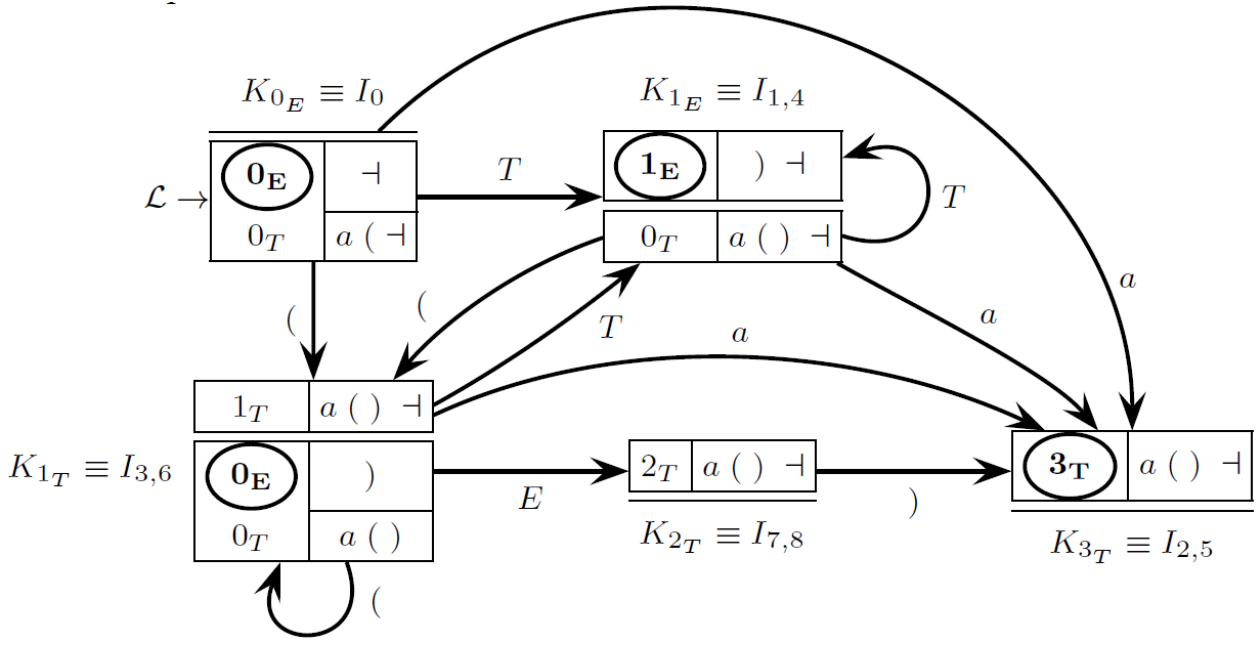
\includegraphics[width=0.6\linewidth]{images/pil1.png}
    \end{figure}
\end{example}

\subsection*{Parser control-flow graph}
The parser control-flow graph (PCFG) is the control unit of the ELL(1) syntax analyzer. 
The prospect sets are included only in the final states to choose whether to exit the machine or to continue with some more moves. 
The call arcs are dashed and labeled with a guide set, that is the set of characters that are expected in the input soon after calling the machine. 
The guide set allows choosing whether: 
\begin{itemize}
    \item Executing one call move. 
    \item Scanning a terminal symbol. 
    \item Executing one of two or more call moves. 
    \item Exiting the machine (if final state).
\end{itemize}
\begin{example}
    Consider the pilot of the previous example. 
    The corresponding parser control-flow graph is as follows: 
    \begin{figure}[H]
        \centering
        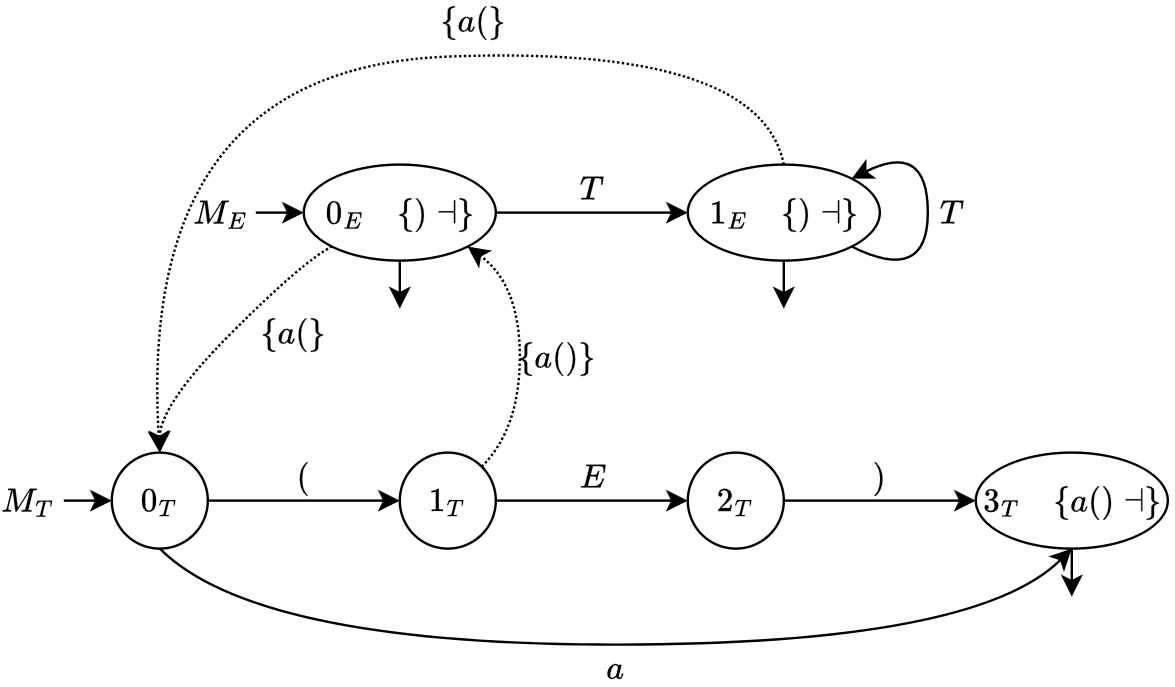
\includegraphics[width=0.6\linewidth]{images/pcfg.png}
    \end{figure}
\end{example}

The character $b$ is in the guide set, denoted as $b \in \textnormal{Gui}(q_A \dashrightarrow 0_{A_1})$, if one of the following properties holds:  
\begin{itemize}
    \item $b \in \textnormal{Ini}(L(0_{A_1}))$. 
    \item $A_1$ is nullable and $b \in \textnormal{Ini}(L(r_A))$. 
    \item $A_1$ and $L(r_A)$ are both nullable and $b \in \pi_{r_A}$.
    \item Exists in $\mathcal{F}$ a call arc $0_{A_1} \overset{\gamma_2}{\dashrightarrow} 0_{A_2}$ and $b \in \gamma_2$. 
\end{itemize}
The guide sets of the call arcs that depart from the same state have to be disjoint from one another, and be disjoint from all the scan arcs from the same state. 

In a PCFG almost all the arcs (except the non-terminal shift) are interpreted as conditional instructions: 
\begin{itemize}
    \item Terminal arcs $p \overset{a}{\rightarrow} q$ run if an only if the current character $cc=a$. 
    \item Call arcs $q_A \rightarrow 0_B$ run if an only if the current character is $cc \in \textnormal{Gui}(q_A \rightarrow 0_B)$. 
    \item Exit arcs (darts) $f_A \rightarrow$ from a state with an item $\left\langle f_A, \pi \right\rangle$ run if and only if the current character is $cc \in \pi$. 
    \item The non-terminal arcs $p \overset{a}{\rightarrow} q$ are interpreted as (unconditioned) return instructions from a machine. 
\end{itemize}
\begin{property}
    If the guide sets are disjoint, then the condition for ELL(1) is satisfied. 
\end{property}

\subsection*{Algorithm}
The stack elements are the states of the PCFG. 
The stack is initialized with element $\left\langle 0_E \right\rangle$. 
Suppose $\left\langle q_A \right\rangle$ is the stack top (it means that machine $M$, is active and in the state $q_A$). 
The ELL syntax analyzer has four move types: 
\begin{itemize}
    \item Scan move: if the shift arc $q_A \overset{cc}{\rightarrow}r_A$ exists, then scan the next token and replace the stack top by $\left\langle r_A \right\rangle$ (the active machine does not change). 
    \item Call move: if there exists a call arc $q_A \overset{\gamma}{\dashrightarrow} 0_B$ such that $cc \in \gamma$, let $q_A \overset{B}{\rightarrow}r_A$ be the corresponding nonterminal shift arc; then pop, push element $\left\langle r_A \right\rangle$ and push element $\left\langle 0_B \right\rangle$.
    \item Return move: if $q_A$ is a final state and token $cc$ is in the prospect set associated with $q_A$, then pop. 
    \item Recognition move: if $M_A$ is the axiom machine, $q_A$ is a final state and $cc =\dashv$, then accept and halt. 
\end{itemize}
In any other case the analyzer stops and rejects the input string.

\subsection*{Parser implementation by means of recursive procedures}
With this implementation the machine becomes a procedure without parameters and, consequently, we have  one procedure per each nonterminal. 
A call move become a procedure call, a can move become a call procedure next, and a return move become a return from procedure. 
Parser Control Flow Graph becomes the control graph of the procedure. 

Use the guide sets and the prospect sets to choose which move to execute. 
The analysis starts by calling the axiomatic procedure. 

\subsection*{Direct construction of the parser control-flow graph}
It is possible to construct the PCFG without building the full ELR pilot graph. 
To do this we simply put call arcs on the machine net and annotate the net with the prospect and guide sets. 

To build the prospect set we have to distinguish between initial states and other states. 
For the initial states $0_A$ we have that: 
\[\pi_{0_A}:=\pi_{0_A} \cup \bigcup_{q_i \overset{A}{\rightarrow} r_i}\left( \textnormal{Ini}(L(r_i)) \cup \textnormal{ if Null}(L(r_i)) \textnormal{ then } \pi_{q_i} \textnormal{ else } \varnothing \right)\]
For every non-initial state we have: 
\[\pi_q:=\bigcup_{p_i \overset{X_i}{\rightarrow}q}\pi_{p_i}\]

To build the guide set we have to apply iteratively this formula: 
\[\textnormal{Gui}(q_A \dashrightarrow 0_{A_1}):=\bigcup
\begin{cases}
    \textnormal{Ini}(L(A_1)) \\
    \textnormal{If Null}(A_1) \textnormal{ then Ini}(L(r_A)) \textnormal{ else } \varnothing \\
    \textnormal{If Null}(A_1) \land \textnormal{Null}(L(r_A)) \textnormal{ then Ini}(\pi_(r_A)) \textnormal{ else } \varnothing \\
    \bigcup_{0_{A_1} \dashrightarrow 0_{B_i}}\textnormal{Gui}(0_{A_1} \dashrightarrow 0_{B_i})
\end{cases}\]
Furthermore (for the final darts and the terminal shift arcs): 
\[\textnormal{Gui}(f_A \rightarrow):=\pi_{f_A}\]
\[\textnormal{Gui}(q_A \overset{a}{\rightarrow}r_A):=\{a\}\]

\subsection*{Modification of grammar not in ELL(1)}
If the ELL(1) condition is not verified, we can try to modify the grammar and make it of type ELL(1).
This approach may take a long time and be a hard work. 

The alternative approach consists in using a longer look-ahead: the analyzer looks at a number $k >1$ of consecutive characters in the input. 
If the guide sets of length $k$ on alternative moves are disjoint, then the ELL(k) analysis is possible.
    \section{Timed languages}

A timed $\omega$-word (or simply timed word) is an infinite sequence of states, where each state is associated with a real-valued timestamp.
Formally, a timed word is a sequence:
\[(\sigma_1,\tau_1),(\sigma_2,\tau_2),(\sigma_3,\tau_3),\dots\]
Here, each symbol $\sigma_i$ is a symbol from a finite alphabet, and $\tau_i$ is a real-valued timestamp indicating when $\sigma_i$ occurs.
\begin{definition}[\textit{Timed sequence}]
    A timed sequence is an infinite sequence of time values:
    \[\tau=\tau_1,\tau_2,\tau_3,\dots\]
    Here, each $\tau_i$ satisfies: 
    \begin{itemize}
        \item \textit{Monotonicity}: $\tau_i\leq\tau_{i+1}$ for all $i\geq 1$. 
            If $\tau_i<\tau_{i+1}$ for all $i\geq 1$ the sequence is strictly monotonic.
        \item \textit{Progress}: for every real number $t\in\mathbb{R}_{\geq 0}$, there exists some $i\geq 1$ such that $\tau_i> t$. 
    \end{itemize}
\end{definition}
\begin{definition}[\textit{Timed word}]
    A timed word over an alphabet $\mathcal{A}$ (a finite set of symbols) is a pair:
    \[\sigma,\tau\]
    Here, $\sigma=\sigma_1\sigma_2\sigma_3\dots$ is an $\omega$-word (an infinite sequence of symbols from $\mathcal{A}$), and $\tau$ is a timed sequence providing the timestamps associated with each symbol.
\end{definition}
\begin{definition}[\textit{Timed language}]
    A timed language over an alphabet $\mathcal{A}$ is a set of timed words over $\mathcal{A}$.
\end{definition}

\paragraph*{Un-time operation}
The un-time operation on a timed language discards the time values associated with symbols.

\begin{definition}
    For a timed language $\mathcal{L}$ over $\mathcal{A}$:
    \[\text{un-time}(\mathcal{L}) = \{ \sigma \in \mathcal{A}^\omega \mid \text{there exists a } \tau \text{ such that } (\sigma, \tau) \in \mathcal{L} \}\]
\end{definition}
\noindent $\text{un-time}(\mathcal{L})$ is a set of $\omega$-words.

\subsection{Timed Automata}
A TA is defined over an alphabet of actions, called the input alphabet. 
It is represented as a tuple:
\[\mathcal{A} = \langle L, \Sigma, C, E, l_0, J, F \rangle\]
\noindent Here:
\begin{itemize}
    \item $L$ is a finite set of locations.
    \item $\Sigma$ is a finite set of input symbols.
    \item $C$ is a finite set of clocks.
    \item $l_0 \in L$ is the initial location.
    \item $E \subseteq L \times B(C) \times \Sigma \times 2^C \times L$ is a set of edges, where $B(C)$ denotes the set of clock constraints.
    \item $J: L \to B(C)$ assigns invariants to locations.
    \item $F \subseteq L$ is the set of final locations.
\end{itemize}
\noindent A timed word is accepted if there exists a path leading infinitely often to a final location.

\begin{definition}[\textit{Run}]
    A run $r_{(\sigma, \tau)}$ over a timed word $(\sigma, \tau)$, where $\sigma = \sigma_1 \sigma_2 \dots$ and $\tau = \tau_1 \tau_2 \dots$ is an infinite sequence:
    \[r_{(\sigma, \tau)} = \langle l_0, \eta_0 \rangle \xrightarrow{\sigma_1, \tau_1} \langle l_1, \eta_1 \rangle \xrightarrow{\sigma_2, \tau_2} \langle l_2, \eta_2 \rangle \dots\]
\end{definition}

Here, $l_i \in L$ and $\eta_i$ are clock valuations satisfying:
\begin{itemize}
    \item \textit{Initialization}: $\eta_0(x) = 0$ for all $x \in C$.
    \item \textit{Transition condition}: for all $i \geq 1$, there exists an edge $e \in E$ such that:
        \[e = \langle l_{i-1}, \gamma_i, \sigma_i, \hat{C}_i, l_i \rangle\]
        Here, $(\eta_{i-1} + (\tau_i - \tau_{i-1}))$ satisfies both $\gamma_i$ and $J(l_{i-1})$, and the clock update is given by:
        \[\eta_i = [\hat{C}_i \mapsto  0](\eta_{i-1} + (\tau_i - \tau_{i-1}))\]
    \item $\eta_i$ satisfies the invariant $J(l_i)$.
\end{itemize}
\noindent The set of locations visited infinitely often in the run is denoted by $\inf(r_{(\sigma, \tau)})$.
A timed word $(\sigma, \tau)$ is accepted by a TA $\mathcal{A}$ if:
\[\inf(r(\sigma, \tau)) \cap F \neq \emptyset\]

\subsection{Timed regular languages}
\begin{definition}[\textit{Timed regular language}]
    A timed regular language is a language accepted by some TA.
\end{definition}
\noindent If $\mathcal{L} \subseteq \mathcal{A}^\omega$ is an $\omega$-regular language, then $\mathcal{L}_t = \{ (\sigma, \tau) \mid \sigma \in \mathcal{L} \}$ is a timed regular language.

\paragraph*{Un-timed languages}
Given a TA that accepts a language $\mathcal{L}$, there exists a Büchi automaton (BA) that accepts $\text{un-time}(\mathcal{L})$.
That is, for any timed regular language $\mathcal{L}$, its un-timed version $\text{un-time}(\mathcal{L})$ is $\omega$-regular.
However, simply removing timing constraints is insufficient. 

\subsection{Properties}
TA are closed under union and intersection but not under complement.
TA cannot be determined.
Non-closure under complement limits automata-based model checking.
Language inclusion and equivalence are undecidable.
Emptiness is decidable by verifying the emptiness of the Region Automaton (similar to the Region TS).

\paragraph*{Continuous time semantics}
TA semantics can be defined over signals instead of timed words.
The standard TS semantics is based on timed words.
LTLs are more naturally interpreted over signals.
Decision problems become harder in continuous-time semantics.

\subsection{Model Checking Timed Automata for Linear Temporal Logic}
Model checking TA for LTL is PSPACE-complete.
The steps are: 
\begin{enumerate}
    \item Construct a Büchi automaton equivalent to the negation of a formula.
    \item Build the product of this Büchi automaton with the TA.
    \item Verify the emptiness of the resulting automaton.
\end{enumerate}
\noindent Since TA are closed under intersection, the result is still a TA.
However, most metric extensions of LTL are undecidable.
    \section{Exercise 6}

Consider the following tables: 
\begin{itemize}
    \item USER(\underline{Email}, Password, LastName, FirstName): contains 128000 users and is stored on 25000 blocks, with a primary hash organization on the primary key.
    \item REVIEW(\underline{Email}, \underline{ISBN}, Date, Rating, ReviewText): has instead 4000000 tuples and is organized with a primary B+ tree with (email, ISBN) as a key; the average fan-out is equal to 35 and leaf nodes occupy 1000000 blocks.
\end{itemize}
Estimate the cost of joining the tables with the best technique.

\paragraph*{Solution}
The lookup cost for the USER table is one since it has a hash indexing. 
In the case of REVIEW we have that each user has an average of 32 reviews (4M/128K). 
Every user also have 9 nodes (1M leaf/128K tuples)
\begin{itemize}
    \item Indexed nested loop with USER as external:
        USER is external, so we have to check all its blocks (25000).
        REVIEW has a cost of 5 based on the levels, but since every user needs to be accessed 9 times (9 blocks associated to each user), we have that the cost for each user is given by the sum of $5-1$ levels and the number of leaf nodes. 
        The total final cost will be: 
        \[25000 + 128000 \cdot (4 + 9) = 1700000\]
    \item Indexed nested loop with REVIEW as external:
        REVIEW is external, so we have to check all its blocks (1000000) after scanning the 4 intermediate nodes, with a total of 1000004.
        In theory, we have to access 4 million tuples, but since the users are only 128000 we can do fewer accesses (all with unitary cost).
        The final cost will be: 
        \[4 + 1000000 + 128000 = 1130000\]
\end{itemize}

    \chapter{Hoare logic}
    \section{Introduction}

Cloud Computing refers to a comprehensive, expansive system of computing, storage, and networking resources that are easily accessible to the public. 
These resources can be accessed through web service calls over the Internet, allowing for short- or long-term usage based on a pay-per-use model.

\subsection{Virtualization}
Virtualization involves partitioning and sharing hardware resources such as CPU and RAM among multiple virtual machines (VMs). 
A virtual machine monitor (VMM) oversees the allocation of physical resources to running VMs, ensuring performance isolation and security.

Without virtualization, software is closely tied to specific hardware, making it challenging to move or modify applications. 
Failures or crashes are typically isolated to individual servers, operating systems, and applications, resulting in low CPU utilization.

With virtualization, software and hardware become independent, offering greater flexibility with pre-built VMs. 
Operating systems and applications can be managed as unified entities, simplifying deployment and management.

The impact of virtualization on IT systems evolution includes server consolidation and the facilitation of cloud computing.

\paragraph*{Server consolidation}
Server consolidation involves migrating from physical to virtual machines. 
This process allows for seamless movement of virtual machines without disrupting the applications running inside. 
Workloads can be automatically balanced based on predefined limits and guarantees, ensuring efficient resource utilization and protecting servers and applications from component and system failures.
The advantages of server consolidation include:
\begin{itemize}
    \item Running different operating systems on the same hardware, leading to higher hardware utilization.
    \item Reduced hardware requirements, resulting in cost savings in acquisition and management (including human resources, power, and cooling), as well as promoting environmentally friendly practices (Green IT).
    \item Continued use of legacy software, such as running Windows applications on Linux machines through virtualization.
    \item Application independence from underlying hardware, providing flexibility and ease of maintenance.
\end{itemize}
    \section{Analytical Customer Relationship Management}

Analytical CRM focuses on leveraging customer data to derive actionable insights, enabling businesses to make informed decisions and enhance customer relationships. 
It encompasses various techniques and processes aimed at understanding customer behavior, predicting trends, and optimizing marketing strategies.

\subsection{Data mining}
Data mining involves the systematic analysis of large datasets to uncover hidden patterns, correlations, and insights that are critical for strategic business management. 
This process can be executed using a variety of techniques, ranging from traditional methods such as descriptive statistics, data visualization, and statistical correlations to more advanced approaches like machine learning algorithms.

These patterns must be presented in an intuitive and interpretable manner to ensure they can be effectively utilized by decision-makers. 
With the growing volume of operational data stored in corporate databases, data mining has become an essential tool for knowledge management, helping organizations unlock valuable insights embedded within their data.

\subsection{Customer profiling}
Customer profiling involves segmenting customers based on identifiable characteristics and behaviors, often facilitated by tools like loyalty cards or transaction histories. 
Customers can be categorized along multiple dimensions, including:
\begin{itemize}
    \item \textit{Loyalty}: analyzing purchasing habits to determine how frequently and consistently customers engage with the brand.
    \item \textit{Price Sensitivity}: assessing how responsive customers are to pricing changes or discounts.
    \item \textit{Lifestyle}: evaluating behavioral orientations across various dimensions, such as preferences, interests, and demographic factors.
\end{itemize}
\noindent Customer segmentation serves as the foundation for targeted marketing efforts. 
By identifying specific segments or combinations of segments, businesses can tailor promotions to align with the average characteristics of each group.
This approach not only enhances the effectiveness of marketing campaigns but also enriches the understanding of individual customer preferences.

\subsection{Campaign management}
Campaign management refers to the set of functionalities designed to support the planning, execution, and evaluation of marketing campaigns. 
A typical campaign lifecycle consists of four key phases, each with its associated tasks and objectives:
\begin{enumerate}
    \item \textit{Planning and budgeting}: defining campaign goals, target audiences, resource allocation, and financial constraints.
    \item \textit{Design}: developing campaign materials, messaging, and strategies to engage the intended audience effectively.
    \item \textit{Execution}: implementing the campaign across selected channels.
    \item \textit{Evaluation}: measuring campaign performance through key metrics.
\end{enumerate}
    \section{Firewall}

\begin{definition}[\textit{Firewall}]
    A firewall is a network security system designed to monitor and control incoming and outgoing network traffic based on predetermined security rules.
\end{definition}
The primary functions of a firewall include:
\begin{itemize}
    \item \textit{IP packet filtering}: examining and controlling packet flow based on IP address and port number.
    \item \textit{Network Address Translation} (NAT): modifying IP address information in packet headers to improve network security and efficiency.
\end{itemize}
A firewall acts as a gatekeeper, enforcing security policies between a protected internal network and external networks.

While firewalls are effective at managing traffic between different networks, they are generally ineffective against insider threats unless the network is properly segmented.
They cannot prevent unauthorized activities originating from within the network itself.

Firewalls are essentially specialized computers and may have vulnerabilities of their own. 
Most firewalls are purpose-built appliances with minimal firmware and limited additional services, reducing their attack surface. 
They enforce security policies by applying rules that should follow a default-deny approach, where all traffic is denied unless explicitly allowed.

Firewalls can be categorized based on their packet inspection capabilities:
\begin{itemize}
    \item \textit{Network layer firewalls}: include packet filters and stateful packet filters that operate at the network layer.
    \item \textit{Application layer firewalls}: include circuit-level gateways and application proxies that operate at the application layer.
\end{itemize}

\subsection{Packet filters}
Packet filters process individual packets by examining IP and part of the TCP headers. 
They are stateless, meaning they do not track the state of TCP connections or fully inspect packet payloads. 
Packet filters, often implemented as Access Control Lists (ACLs) on routers, base their decisions on packet-specific conditions such as IP addresses and port numbers.

\subsection{Stateful packet filters}
Stateful packet filters build upon basic packet filtering by tracking the state of active TCP connections. 
They ensure packets follow the correct sequence and provide more robust security.
While they offer deeper inspection and additional features such as NAT, packet defragmentation, and reassembly, they can also impact performance due to their connection-oriented nature.

\subsection{Circuit firewalls}
Circuit firewalls function as TCP-level proxies. 
They relay TCP connections by allowing clients to connect to a specific port on the firewall, which then establishes a connection to the desired server on behalf of the client.

\subsection{Application proxies}
pplication proxies operate at the application layer, inspecting, validating, and modifying protocol data. 
They provide additional features such as user authentication, specific filtering policies, advanced logging, and content filtering. 
Application proxies may require modifications to clients and servers to function properly.

\subsection{Multi-zone architecture}
Traditional perimeter defense strategies often assume that once external threats are blocked, the internal network remains secure. 
However, this assumption is challenged by scenarios such as remote access to resources and remote user access to corporate networks. 
These scenarios can compromise internal network security by mixing externally accessible servers with internal clients.

A robust approach to addressing these security concerns is the implementation of a multi-zone architecture. 
This approach divides the network into distinct zones based on privilege levels and uses firewalls to control access between them. 
A key component of this architecture is the creation of a Demilitarized Zone (DMZ) where public-facing servers are placed. 
The DMZ is considered a high-risk area similar to the internet, and critical data and systems are kept separate from it.

\paragraph*{Virtual Private Network}
Virtual Private Networks (VPN) allow remote employees to securely access corporate resources and connect remote sites without requiring dedicated leased lines. 
They ensure the confidentiality, integrity, and availability (CIA) of data over public networks by creating encrypted connections. 
VPNs support two main types of tunneling:
\begin{itemize}
    \item \textit{Full tunneling}: all traffic is routed through the VPN, which allows comprehensive control over security policies and traffic monitoring.
    \item \textit{Split tunneling}: only traffic intended for the corporate network is routed through the VPN, while other traffic goes directly to the internet. 
        This method can improve efficiency but reduces control over non-corporate traffic.
\end{itemize}
    \section{Dialog systems evaluation}

Evaluating dialogue systems remains a complex and evolving challenge. 
Unlike task-specific models, open-domain conversational agents must be assessed across multiple dimensions of quality—many of which are inherently subjective and difficult to measure automatically.
Eight commonly considered dimensions of quality in dialogue include: repetition, interestingness, coherence, fluency, listening, inquisitiveness, humanness, and engagingness. 

\subsection{Human evaluation}
Human assessments are essential for gauging subjective aspects of quality. 
These evaluations are typically divided into two formats:
\begin{itemize}
    \item \textit{Participant evaluation}: users interact with the system and then answer targeted questions.
    \item \textit{Observers evaluation}: annotators compare pairs of conversations and assess them along qualitative axes. 
\end{itemize}
\noindent These comparative judgments often provide more reliable insight than absolute scoring.

\subsection{Automatic evaluation}
Automatic evaluation of dialogue systems remains an open research problem.
Traditional metrics from fields like machine translation are rarely used in conversational AI because they show low correlation with human judgments, and fail to capture contextual appropriateness, tone, or relevance in conversation.
The main alternative approaches are: 
\begin{itemize}
    \item \textit{Adversarial evaluation}: inspired by the Turing Test, this method trains a classifier to distinguish between human and machine responses.
         The more the model can fool the classifier, the better its perceived quality.
    \item \textit{LLM-as-a-judge}: these models are prompted to score or rank conversations based on quality dimensions—offering scalable, semi-automated evaluation with surprisingly strong alignment to human preferences.
\end{itemize}
\noindent For systems built to accomplish specific tasks evaluation focuses more on functional success such as: end-to-end task success, slot error rate, user studies, efficiency, and system robustness.
\end{document}